\documentclass[sigconf]{acmart}
\settopmatter{printacmref=true}

%%
%% \BibTeX command to typeset BibTeX logo in the docs
\AtBeginDocument{%
	\providecommand\BibTeX{{%
			\normalfont B\kern-0.5em{\scshape i\kern-0.25em b}\kern-0.8em\TeX}}}

%% Rights management information.  This information is sent to you
%% when you complete the rights form.  These commands have SAMPLE
%% values in them; it is your responsibility as an author to replace
%% the commands and values with those provided to you when you
%% complete the rights form.
%\setcopyright{acmcopyright}
%\copyrightyear{2020}
%\acmYear{2020}
%\acmDOI{10.1145/1122445.1122456}

%% These commands are for a PROCEEDINGS abstract or paper.
%\acmConference[CIKM '20]{The 29th ACM International Conference on Iformation and Knowledge Management}{October  19--23, 2020}{Galway, Ireland}
%\acmBooktitle{The 29th ACM International Conference on Information and Knowledge Management (CIKM '20), October 19--23, 2020, Galway, Ireland}
%\acmPrice{15.00}
%\acmISBN{978-1-4503-XXXX-X/18/06}

\copyrightyear{2020}
\acmYear{2020}
\setcopyright{acmcopyright}\acmConference[CIKM '20]{Proceedings of the 29th ACM International Conference on Information and Knowledge Management}{October 19--23, 2020}{Virtual Event, Ireland}
\acmBooktitle{Proceedings of the 29th ACM International Conference on Information and Knowledge Management (CIKM '20), October 19--23, 2020, Virtual Event, Ireland}
\acmPrice{15.00}
\acmDOI{10.1145/3340531.3411858}
\acmISBN{978-1-4503-6859-9/20/10}


%\usepackage{times}
\usepackage{soul}
\usepackage{url}
\usepackage[utf8]{inputenc}
\usepackage{graphicx}
\usepackage{amsmath}
\usepackage{amsthm}
\usepackage{booktabs}
\usepackage{algorithm}
\usepackage{algorithmic}
\usepackage{bm}
\usepackage{tabu}
\usepackage{diagbox}
\usepackage{mathrsfs}
%\usepackage[noend]{algpseudocode}
\usepackage{amsfonts}
%\usepackage{AMSFonts}
%\usepackage{amssymb}
\usepackage{multirow, multicol}
\urlstyle{same}
\usepackage{CJKutf8}
\usepackage{color}
\usepackage{subfigure}

% the following package is optional:
%\usepackage{latexsym}

\newtheorem{example}{Example}
\newtheorem{theorem}{Theorem}
\newcommand{\KZ}[1]{\textcolor{blue}{Kenny: #1}}
\newcommand{\figref}[1]{Figure \ref{#1}}
\newcommand{\eqnref}[1]{Eq. \ref{#1}}
\newcommand{\tabref}[1]{Table \ref{#1}}
\newcommand{\secref}[1]{Section \ref{#1}}
\newcommand{\algoref}[1]{Algorithm \ref{#1}}


\begin{document}
\fancyhead{}
	
\title{MICK: A Meta-Learning Framework for Few-shot Relation Classification with Small Training Data}

\author{Xiaoqing Geng}
\email{gxq961127@sjtu.edu.cn}
\affiliation{%
	\institution{Shanghai Jiao Tong University}
}
\author{Xiwen Chen}
\email{victoria-x@sjtu.edu.cn}
\affiliation{%
	\institution{University of Michigan-Shanghai Jiao Tong University Joint Institute}
}
\author{Kenny Q. Zhu}
\authornote{Corresponding Author.}
\email{kzhu@cs.sjtu.edu.cn}
\affiliation{%
	\institution{Shanghai Jiao Tong University}
}
\author{Libin Shen}
\email{libin@leyantech.com}
\affiliation{%
	\institution{Leyan Tech}
}
\author{Yinggong Zhao}
\email{ygzhao@leyantech.com}
\affiliation{%
	\institution{Leyan Tech}
}

\begin{CJK}{UTF8}{gkai}
	
\begin{abstract}
Few-shot relation classification seeks to classify incoming query instances after meeting 
only few support instances. % during testing.
This ability is gained by training with large amount of in-domain annotated data. 
In this paper, we tackle an even harder problem by further limiting the amount of data available
at training time. 
%In this paper, 
We propose a few-shot learning framework for %sentence-based 
relation classification,
which is particularly powerful when the training data is very small.
In this framework, models not only strive to classify query instances, but also seek 
underlying knowledge about the support instances
to obtain better instance representations. %models are trained not only by queries but also the support instances.
The framework also includes a method for aggregating cross-domain knowledge into models by 
open-source task enrichment.
Additionally, we construct a brand new dataset: the TinyRel-CM dataset, a few-shot relation 
classification dataset in health domain with purposely small training data
and challenging relation classes. Experimental results demonstrate that our framework brings
performance gains for most underlying classification models,
%\KZ{I think you are talking about underlying classification models?}
outperforms the state-of-the-art results given small training data, 
%(e.g., on TinyRel-CM dataset and FewRel-dataset \cite{han-etal-2018-fewrel} with 
%shrunken training data), 
and achieves competitive results with sufficiently large training data.
%(e.g., on FewRel dataset with full training data).
%on TinyRel-CM dataset and achieves competitive results on
%the FewRel dataset \cite{han-etal-2018-fewrel}, especially when extremely small amount of training data is given.
% \KZ{Don't mention MESDA everywhere, but only when you need to refer to it succinctly.}
\end{abstract}


%%
%% The code below is generated by the tool at http://dl.acm.org/ccs.cfm.
%% Please copy and paste the code instead of the example below.
%%
%%
%% Keywords. The author(s) should pick words that accurately describe
%% the work being presented. Separate the keywords with commas.
\keywords{few-shot learning, meta-learning, small training data, relation classification}


%%
%% This command processes the author and affiliation and title
%% information and builds the first part of the formatted document.
\maketitle

\section{Introduction}
% What is RC. Given sufficient data good, otherwise bad.
Relation classification(RC) is an indispensable problem in natural language processing(NLP). Given a sentence (e.g., \emph{Washington is the capital of the United States}) containing two entities we focus on (e.g., \emph{Washington} and \emph{the United States}), an RC model aims to distinguish the semantic relation between the entities conveyed by the sentence (e.g., \emph{capital of}).

Conventional relation classification has been an extensively investigated task. Recent approaches substantially base on neural networks and deep learning \citep{RecursiveNNRC, zeng-etal-2014-relation, RNNRC, vu-etal-2016-combining}, where the models are trained with sufficient human-annotated data and achieve satisfactory results.
%\KZ{What does this mean? OK}
However, human-annotation is expensive. It is burdensome to attain considerable amount of labeled data, under which circumstance a sharp decrease occurs in the performance of conventional RC models.
% Distant supervised ways
Distant supervised methods have been adopted to enlarge annotation quantity by utilizing existing knowledge bases to perform auto-labeling on massive raw corpus. The NYT-10 dataset \citep{NYTdataset} is a typical large dataset constructed under distant supervision. Although distance supervised approaches greatly augment labeled data, significant shortcomings expose: %\KZ{Elaborate a bit what you mean bylong-tail problem. OK}
(1) Long-tail problems \citep{xiong-etal-2018-one, han-etal-2018-fewrel, ye-ling-2019-multi} exist in knowledge bases. While some particular relation classes contain a great proportion of instances, most classes consist of only tens of instances.  (2) Noise issues occur during auto-labeling, demanding for manual screening.

% Few-shot RC
Few-shot relation classification is a particular RC task under minimum annotated data. In few-shot relation classification tasks, a model is required to distinguish the category of a new incoming query instance given only few support instances (e.g., 5 or 10). An example is given in Table~\ref{FewShotRCExample}.

\begin{table}[t]
\centering
\small
\begin{tabular}{p{7.3cm}}
\hline
\textbf{Support Set} \\ \hline
\textbf{Class1} \emph{~mother}: \\
\qquad \textbf{Instance1}~\lbrack Emmy Acht\'e\rbrack$_{entity1}$ was the mother of the internationally famouse opera singers \lbrack Aino Ackt\'e\rbrack$_{entity2}$ and Irma Tervani. \\
\qquad \textbf{Instance2}~He was deposed in 922, and \lbrack Eadgifu\rbrack$_{entity1}$ sent their son, \lbrack Louis\rbrack$_{entity2}$ to safety in England. \\
\qquad \textbf{Instance3}~Jinnah and his wife \lbrack Rattanbai Petit\rbrack$_{entity1}$ had separated soon after their daughter, \lbrack Dina Wadia\rbrack$_{entity2}$ was born. \\
\qquad \textbf{Instance4}~Ariston had three other children by \lbrack Perictione\rbrack$_{entity1}$: Glaucon, \lbrack Adeimantus\rbrack$_{entity2}$, and Potone.\\
\qquad \textbf{Instance5}~She married (and murdered) \lbrack Polyctor\rbrack$_{entity2}$, son of Aegyptus and \lbrack Caliadne\rbrack$_{entity1}$. Apollodorus.\\
\textbf{Class2} \emph{~spouse}: ... \\
\textbf{Class3} \emph{~child}: ... \\
\textbf{Class4} \emph{~follows}: ... \\
\textbf{Class5} \emph{~crosses}: ... \\ \hline
\textbf{Query Instance} \\ \hline
Dylan and \lbrack Caitlin\rbrack$_{entity1}$ brought up their three children, \lbrack Aeronwy\rbrack$_{entity2}$, Llewellyn and Colm. \\
\hline
\end{tabular}
\caption{\label{FewShotRCExample}
An example of 5 way 5 shot relation classification scenario from the FewRel \citep{han-etal-2018-fewrel} validation set. The query instance is of Class1:\emph{mother}. The support instances of Class2-5 are omitted.
}
\end{table}

% Meta learning
Meta-learning is a major method under few-shot learning circumstances and is broadly studied in computer vision (CV) \citep{LakeHuman, Santoro2016, proto}. Instead of training a neural network to learn a specific task, in meta-learning, the model is trained with a variety of similar but different tasks to gain the ability of quick adaptation to new tasks without meeting a ton of data.
One framework of meta-learning is to train an additional meta-learner %
%\KZ{Rephrase this: on the upper to guide the upgrading steps of the conventional learner on the lower OK}
which sets and adjusts the update rules for the conventional learner \citep{Andry2016, Finn2017, HN}. Another bases on metric learning and is aimed at the acquisition of distance distribution among the relations \citep{Koch2015, Vinyals2016, proto}.
%Prototypical networks \citep{proto} is a typical and widely used metric learning based meta-learning framework.

% Recent works on meta-RC
In recent years, meta-learning has been adopted in NLP as solutions to multiple few-shot learning tasks \citep{gu-etal-2018-meta, han-etal-2018-fewrel, huang-etal-2018-natural, obamuyide-vlachos-2019-meta, ye-ling-2019-multi}. In this paper, we focus on meta-learning methods on few-shot relation classification task.
 \citet{han-etal-2018-fewrel} constructed the FewRel dataset and first applied distinct meta-learning frameworks intended for CV tasks on the FewRel dataset. Prototypical networks \citep{proto} with CNN encoder turned out to have the best performance. \citet{ye-ling-2019-multi} improved the framework of prototypical networks by interactively encoding the support and query instances at both local and instance level, and adding weights while calculating prototypes.

% What's different in our work
Admitting that meta-learning frameworks outperform conventional methods in few-shot relation classification, we see room for further improvements.
Firstly, the previous models concern much about
%\KZ{the outputs of the query instances OK}
computations on query instances but lose sight of the significance of information within the support instances. Secondly, the demand for much human annotation is not \emph{really} settled in previous works. Even though just few support instances are needed during testing, the training set is still sufficient and large (e.g., the FewRel dataset \citep{han-etal-2018-fewrel} contains 700 instances per relation). And performance drops when the training data size is restricted (e.g., tens of instances per relation).

Our proposed
%\KZ{Find another name?}
\emph{Metric-learning based Meta-learner Enhanced} (MME) meta-learning framework improves these weaknesses. Firstly, in MME, to exploit the underlying knowledge within support instances, we add a supplementary classifier over the support instances which contributes to the update of the model by a unique fast-slow learner strategy. Secondly, we show that meta-learning is capable of learning cross-domain underlying knowledge and we improve the model performance by augmenting training data with open-source relation classification instances. This is extremely helpful under circumstances where few training data of the target domain is available.

Additionally, we propose our own dataset, \emph{Few-shot Relation-classification Medical} (FRM) dataset, a Chinese few-shot relation classification dataset in medical domain. The FRM dataset contains 27 relations with 50 instances per relation. Experiments are conducted on both our proposed FRM dataset and the FewRel dataset \citep{han-etal-2018-fewrel}. Experimental results show that (1)
%\KZ{How do you show it's a hard task? OK}
The FRM dataset provides a hard task. Strong baselines behave poorly on the FRM dataset. (2) Our proposed MME framework works out to have the best performance on FRM dataset and achieves competitive results on the FewRel dataset.

% Our contributions
In summary, our contributions include: (1) We propose a novel \emph{Metric-learning based Meta-learner Enhanced} (MME) meta-learning framework which fully utilize the information brought in support instances with the help of a supplementary classifier and a meta-learner. (2) We illustrate that meta-learning process learns cross domain underlying knowledge and propose an approach to add supplementary data during training process to achieve performance gains. (3) We propose \emph{Few-shot Relation-classification Medical} (FRM) dataset, a Chinese few-shot relation classification dataset in medical domain. (4) Our approach achieves state-of-the-art performance on FRM dataset and competitive results on FewRel \citep{han-etal-2018-fewrel} dataset.


\section{Problem Formulation}
%\KZ{Don't use the term constraint so much: constraint is usually a more complex mathematical
%equation or inequality. Here it's just simply a limitation.} 
We add limitation on the size of training data compared with previous few-shot relation classification tasks.
Just like in conventional few-shot relation classification, there is a training set
$D_{\rm{train}}$ and a test set $D_{\rm{test}}$.
Each instance in both sets can be represented as a triple $(s,e,r)$,
where $s$ is a sentence of length $T$, $e=(e_1, e_2)$ is the head and tail entities and
$r$ is the semantic relation between $e_1$ and $e_2$ conveyed by $s$.
$r \in R$, where $R=\{r_1,...,r_N\}$ is the set of all candidate relation classes.
$D_{\rm{train}}$ and $D_{\rm{test}}$ have disjoint relation sets, i.e.,
if a relation $r$ appears in a triple of the training set, it must not appear
in any triples of the test set and vice versa.
$D_{\rm{test}}$ is further split into a support set $D_{\rm{test\text{-}s}}$
and a query set $D_{\rm{test\text{-}q}}$. The problem is to predict
the classes of instances in $D_{\rm{test\text{-}q}}$ given
$D_{\rm{test\text{-}s}}$ and $D_{\rm{train}}$. While no restrictions are lied on how to use $D_{\rm{train}}$, it is conventionally splited into a support set and a query set to train models.
In a $N$-way $K$-shot %few-shot relation classification 
scenario,
$D_{\rm{test\text{-}s}}$ contains $N$ relation classes and $K$ instances
for each class. Both $N$ and $K$ are supposed to be small (e.g., 5-way 1-shot, 10-way 5-shot).
Particularly, we limit the size of training data (i.e.,  $D_{\rm{train}}$ is also small).
The difficulty of 
%few-shot relation classification 
the task lies in not only the small size of
$D_{\rm{test\text{-}s}}$ (totally $N\times K$ instances) but also the small training data size.

%Basing on few-shot relation classification task, we put forward the challenge of few-shot relation classification
%\emph{under limited amount of training data} (i.e., the size of $D_{\rm{train}}$ is also small).
%The small training data size makes the task much harder. %The task becomes harder if the size of $D_{\rm{train}}$ is also small, and


%\section{The FRM Dataset}
In this section, we describe the detailed procedure of constructing \emph{Few-shot Relation-classification Medical} (FRM) dataset and show the dataset statistics. The whole procedure consists of three steps (Figure \ref{fig:construct}): (1) We crawl data from Chinese health-related websites to form a large corpus and an entity dictionary. (2) We automatically align the entities in the corpus with the entity dictionary, forming a large candidate-sentence set. (3) We manually filter out the unqualified candidate sentences and tag qualified ones with corresponding relation labels. Finally, we get a clean Chinese few-shot relation classification dataset in medical domain.

\begin{figure}
    \centering
    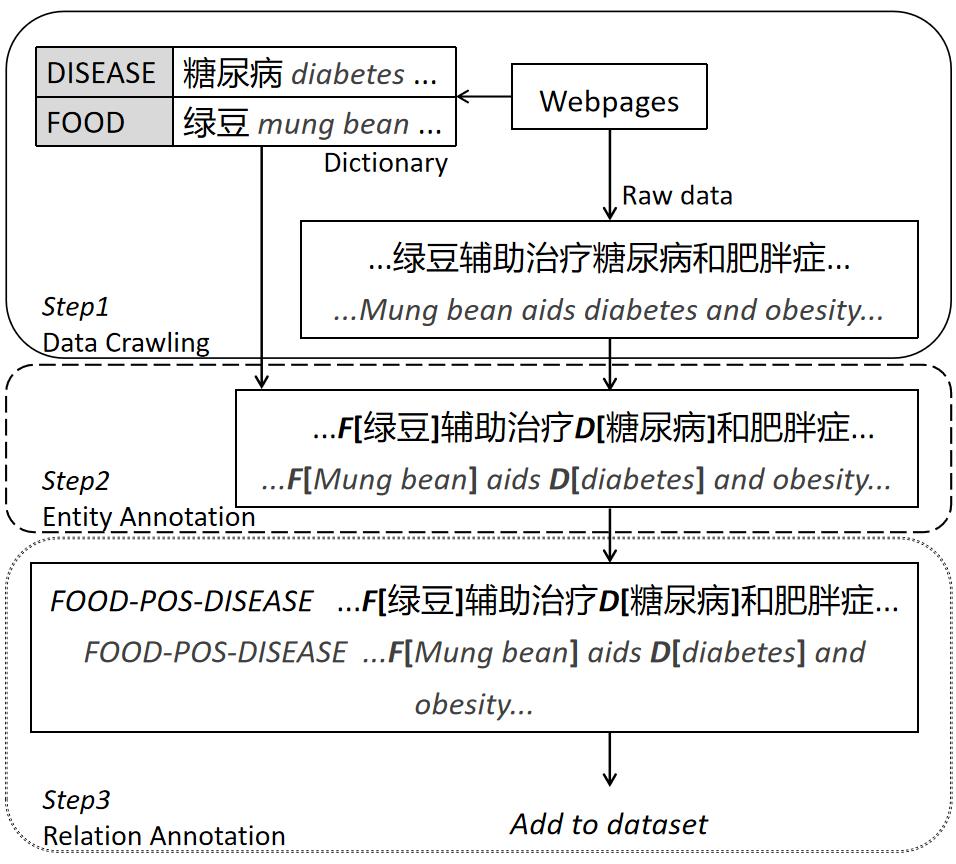
\includegraphics[width=8cm]{datasetconstruct.png}
    \caption{The construction procedure of FRM dataset.}
    \label{fig:construct}
\end{figure}

\subsection{Crawling Corpus and Entity Dictionaries}
The first step of constructing the FRM dataset is to obtain a Chinese medical corpus of considerable size and a dictionary containing different types of entities. Both the corpus and the dictionary is acquired by crawling Chinese health-related websites (\url{http://www.xywy.com},  \url{http://www.39.net} and \url{https://www.9939.com}). An example sentence from the crawled corpus and example entities from dictionaries are shown in Figure \ref{fig:construct} enclosed by the solid rectangle.
\subsection{Auto-labeling Entities}
We automatically align the entities in the dictionary to the sentences in corpus.

We firstly apply longest-exact match to extract sentences that contain two entities in the dictionary. In the longest-exact match procedure, for a candidate string $s$, we denote a substring of length $l$ starting from the $i^{th}$ character as $s_{i,l}$. We adopt a boolean function $m$ where $m(s_{i,l})=True$ if substring $s_{i,l}$ exactly matches an entity in the dictionary, and $False$ otherwise. We go through $s$ from left to right. If $m(s_{i,l})=True$ and there is no $s_{j,k}$ that satisfies (1) $s_{j,k}$ contains $s_{i,l}$ (2)$m(s_{i,l})=True$, we call $s_{i,l}$ a longest matched substring. If a sentence contains two distinct longest matched substrings, we label these two substrings as entities $e$ and add this sentence to a set of candidate sentences.

Then, for each candidate sentence $s$ with entities $e$ labeled, we perform word segmentation on $s$ to split it into words $\{w_0,w_1,...,w_t\}$ where $t$ is the length of the sentence. We assert that for either entity $e_i,i=0,1$ in $e$, it must satisfies $e_i=join(w_j,...w_k)$ for $\forall j,k \in [0...t-1]$ where $join$ is a string joining function. If the requirement is not met, we discard this sentence. Thus only sentences with $e$ that are compete words remain. Example is shown in Figure \ref{fig:construct} the dashed rectangle.
\subsection{Manual Screening and Relation-labeling}
We manually screen out the remaining entity-wrongly-labeled candidate sentences. For each correctly-labeled sentence $s$, we manually tag the relation $r$ to the sentence. Thus we get a triple $(s,e,r)$ and add the triple into the dataset. Example is shown in the dotted rectangle in Figure \ref{fig:construct}.
Relations are manually annotated because of the noise in the crawled sources and the semantic ambiguity issues.
\subsection{Dataset Statistics}


\begin{table}[ht]
\centering
\small
\begin{tabu}{|c|[0.5pt]l|}
\hline
\textbf{Group} & \textbf{Relations} \\ \tabucline[0.5pt]{-}
D-D & complication, cause, is, include, NA \\ \hline
D-S & have, NA\\ \hline
D-F & positive, negative, forbid, prevent, cause, NA\\ \hline
D-N & positive, negative, prevent, lack, cause, NA\\ \hline
F-N & contain, NA\\ \hline
S-F & forbid, cause, positive, negative, prevent, NA\\ \hline
\end{tabu}
\caption{Entity groups in FRM dataset. D,S,F,N stands for Disease, Symptom, Food and Nutrient respectively.}
\label{Egroup}
\end{table}

The FRM dataset contains 27 relations with 50 instances per relation. The 27 relations cover binary relations among 4 entity types. The average length of a sentence in FRM dataset is 67.62, and there are totally 2,187 unique characters.

The 27 relations in FRM dataset can be aggregated into 6 groups according to the entity types (Table \ref{Egroup}). We use separated relations for training and testing. More meaningfully, when treating one group of relations as the test set, other groups serve as the training set. Thus, we can formulate 6 different few-shot relation classification tasks with our FRM dataset.

\begin{table}[ht]
\centering
\small
\begin{tabular}{|l|r|r|r|}
\hline
\textbf{Dataset} & \textbf{\#cls.} & \textbf{\#inst./cls.} & \textbf{\#inst.} \\ \hline
FewRel & 100 & 700 & 70,000 \\ \hline
FRM & 27 & 50 & 1,350 \\ \hline
\end{tabular}
\caption{Comparison of FRM dataset to other few-shot relation classification datasets.}
\label{Datasetcompare}
\end{table}


The FRM dataset provides hard tasks for several reasons. Firstly, we shrink the training data size. Table \ref{Datasetcompare} shows the comparison of data size with previous few-shot relation classification datasets. Secondly, the relations in a given test set are relative to each other since the share common entity types (because the relations are from the same group). In other datasets, the entity types are distinct in most situations, which may serve as extra information. %Figure xx shows example instances from previous datasets and the HEALTHXX dataset. For previous datasets, the instances within the same category is likely to be quite similar while instances from different categories distinct from one to another. While in HEALTHXX datasets, the format of instances within one category varies from one to another, which makes the task harder.

The detailed meaning and example instances of each relation is listed in Appendix ...


\section{Methodology}
In this section, we outline the methodology employed to gather, process, and annotate the data for our study. We begin by detailing the sources of our multimodal video data and personality labels, focusing on how we efficiently align subtitles with original scripts to ensure accurate temporal and character associations. And we also present our annotation process, explaining how we leverage the ChatGPT API to automatically annotate social and emotional relations among characters within the text data. 
\subsection{Source of Data}
Our data source contains mainly two parts, the multimodal video data and personality labels. For video data, we include 14 different genres of TV series and movies via an open-source website\footnote[1]{https://yts.mx/}, and for the scripts and subtitles, we also find other open-source websites\footnote[2]{https://www.simplyscripts.com/}\footnote[3]{https://subscene.com/} for research offering the free scripts and subtitles of many famous movie and television programs. Considering the insufficient labeling method of existing works, we collect the personality annotations from personality database website as well as the voting distribution and align them to correctly scripts. 
\subsection{Data Alignment Process}
As subtitle contain temporal information and original scripts associate utterances with characters, we are supposed to align them properly as efficient as possible. However, most of the existing multimodal datasets annotate the timestamps manually with taking up a great deal of time. There are also some works which utilize different automatic tools to align the utterances with their corresponding information. For instance, \cite{lian2024merbench} use an Automatic Sound Recognition (ASR) tool called Gentle\footnote[4]{https://github.com/lowerquality/gentle} to get the timestamps for the utterances. To streamline the process of aligning dialogue utterances with their respective timestamps and speakers from subtitles, we propose an efficient method leveraging a fuzzy matching algorithm. 
Following successful alignment, we proceed to segment the video content into distinct scenes according to the timestamps. Besides, we use FFmpeg\footnote[5]{https://ffmpeg.org/} to extract the audio track from the video clips and output it as a \textit{.mp3} file.


\begin{figure}[ht]
    \small
    \centering 	 	 	 	
    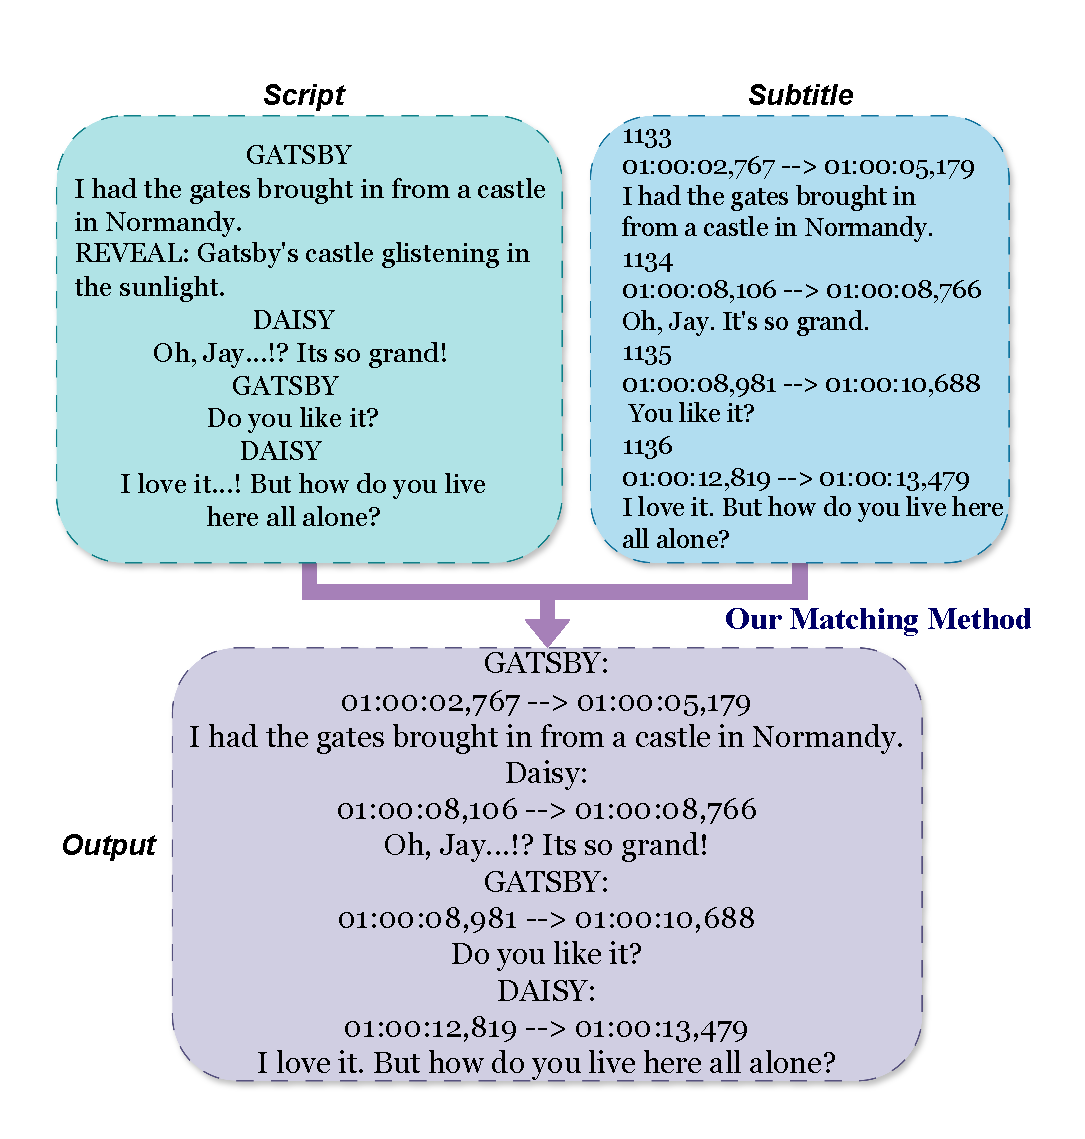
\includegraphics[width=\linewidth, trim= 0 10 0 10, clip]{images/raw_data.pdf}
	\caption{Process of data alignment}
    \label{fig:alig}
\end{figure}

\subsection{Annotation Process}

We developed a process to automatically annotate social and emotional relationships among characters using the ChatGPT API, specifically the \textit{gpt-3.5-turbo-1106} model, which is suited for processing text data. After preprocessing the text and dividing it into scenes, we designed prompts (Fig \ref{fig:prompt}) for ChatGPT to identify social and emotional relationships in each scene. A challenge arose in representing unidirectional affectionate relationships, where one character (A) likes another (B) but the feeling is not mutual. While social relationships are straightforward, emotional relationships require a method to capture this directionality. We addressed this by interpreting the relative position of characters in the tuple: for instance, "A and B (family, fondness)" indicates that A has positive feelings towards B, whereas "B and A (family, fondness)" indicates the opposite. This method effectively captures and represents the directionality of emotional relationships.

\begin{figure}[ht]
	\centering
	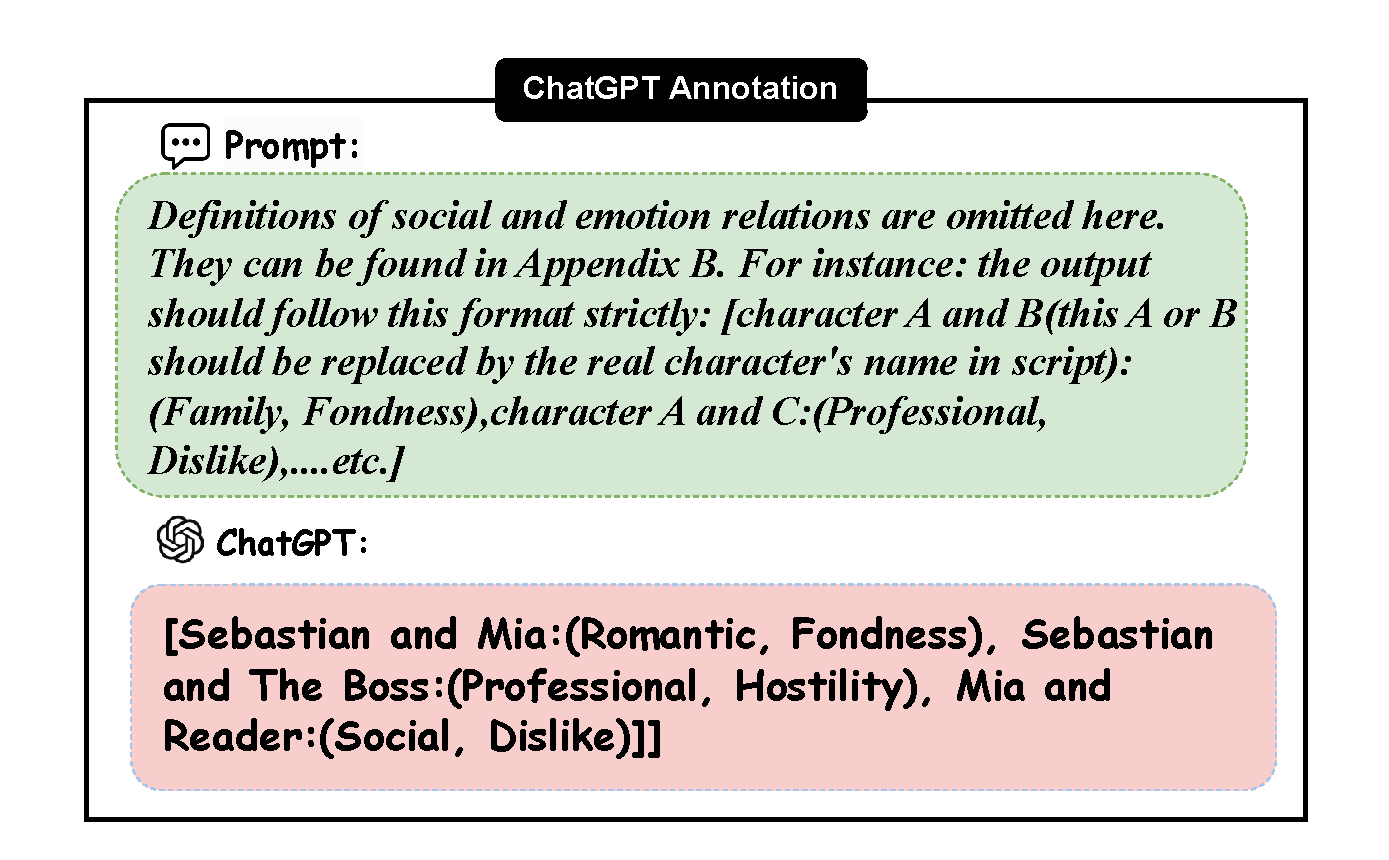
\includegraphics[width=\linewidth]{images/prompt.pdf}
	\caption{Prompt design for relations annotation}
	\label{fig:prompt}
\end{figure}



\section{Experiments}
\label{exp}
In Section \ref{exp}, we explain the experiment process in detail, including datasets, experimental setup, implementation details and evaluation results.

\subsection{Dataset}
\label{dataset}
Experiments are done on two datasets: FewRel dataset \cite{han-etal-2018-fewrel} and our proposed TinyRel-CM dataset.
~\\
~\\
\textbf{FewRel Dataset} FewRel dataset \cite{han-etal-2018-fewrel} is a few-shot relation classification dataset constructed through distant supervision and human annotation. It consists of 100 relation classes with 700 instances per class. The relation classes are split into subsets of size 64, 16 and 20 for training, validation and testing, respectively.
The average length of a sentence in FewRel dataset is 24.99, and there are 124,577 unique tokens in total. At the time of writing, FewRel is the only few-shot relation classification dataset available.
~\\
~\\
\textbf{TinyRel-CM Dataset}\footnote{Code and dataset released in \url{https://github.com/XiaoqingGeng/MICK}.} TinyRel-CM dataset is our proposed Chinese few-shot relation classification dataset in health domain with small training data. The TinyRel-CM dataset is constructed through the following steps: (1) Crawl data from Chinese health-related websites\footnote{\url{www.9939.com}, \url{www.39.net}, and \url{www.xywy.com}} to form a large corpus and an entity dictionary. (2) Automatically align entities in the corpus with the entity dictionary, forming a large candidate-sentence set. (3) 5 Chinese medical students manually filter out the unqualified candidate sentences and tag qualified ones with corresponding class labels to form an instance. An instance is added to the dataset only if 3 or more annotators make consistent decisions. This process costs 4 days.

The TinyRel-CM Dataset consists of 27 relation classes with 50 instances per class. The 27 relation classes cover binary relations among 4 entity types, and are grouped into 6 categories according to the entity types, forming 6 tasks with one group being the test set and other 5 groups serving as training set (see Table \ref{Egroup}). Grouping makes TinyRel-CM dataset more challenging because all candidate relation classes during testing are highly similar. An example instance in the TinyRel-CM dataset is shown in Tabel \ref{FRMexample}. The average length of a sentence in TinyRel-CM dataset is 67.31 characters, and there are 2,197 unique characters in total. Comparison between TinyRel-CM dataset and FewRel dataset is shown in Table \ref{Datasetcompare}.

\begin{table}[ht]
\centering
\small
\caption{Entity groups in TinyRel-CM dataset. D,S,F, and U stand for Disease, Symptom, Food, and nUtrient, respectively.}
\label{Egroup}
\begin{tabu}{|c|[0.5pt]l|}
\hline
\textbf{Group} & \textbf{Classes} \\ \tabucline[0.5pt]{-}
D-D & complication, cause, is, include, NA \\ \hline
D-S & have, NA\\ \hline
D-F & positive, negative, forbid, prevent, cause, NA\\ \hline
D-U & positive, negative, prevent, lack, cause, NA\\ \hline
F-U & contain, NA\\ \hline
S-F & forbid, cause, positive, negative, prevent, NA\\ \hline
\end{tabu}
\end{table}

\begin{table}[ht]
\centering
\small
\caption{An example instance in the TinyRel-CM dataset.}
\label{FRMexample}
\begin{tabular}{|l|p{170pt}|}
\hline
\textbf{Group} & D-D \\ \hline %\tabucline[1pt]{-}
\textbf{Class} & complication \\ \hline
\textbf{Explanation} & Entity 2 is a complication of entity 1. \\ \hline
\multirow{2}{*}{\textbf{Example}} & [子宫肌瘤]$_{entity1}$出现了[慢性盆腔炎]$_{entity2}$并发症,导致月经量过多。 \\
& \textcolor[rgb]{0.45,0.45,0.45}{Once [Hysteromyoma]$_{entity1}$ is complicated with [chronic pelvic inflammation]$_{entity2}$, menstruation increases.}  \\ \hline
\end{tabular}
\end{table}


\begin{table}[ht]
\centering
\small
\caption{Comparison of TinyRel-CM dataset to FewRel dataset.}
\label{Datasetcompare}
\begin{tabular}{|l|r|r|r|}
\hline
\textbf{Dataset} & \textbf{\#cls.} & \textbf{\#inst./cls.} & \textbf{\#inst.} \\ \hline
FewRel & 100 & 700 & 70,000 \\ \hline
TinyRel-CM & 27 & 50 & 1,350 \\ \hline
\end{tabular}
\end{table}


%The TinyRel-CM dataset is harder than FewRel dataset for two reasons. On one hand, the training data size is small (as is shown in Table \ref{Datasetcompare}). On the other hand, under each task, the candidate relation classes are relative to each other since they share common entity types (because the classes are from the same entity group). For example, a model needs to choose the correct relation class for the example instance in Table \ref{FRMexample} among classes \emph{Disease-complication-Disease, Disease-cause-Disease, Disease-is-Disease, etc.}.
%In FewRel dataset, the head and tail entity types are distinct in most of the cases (see Table~\ref{FewShotRCExample}), making the relation classes easier to distinguish.
%The difference in entity types may also
%%serve as extra information,
%mislead the models into learning to distinguish entity types instead of relation classes.
%%Figure xx shows example instances from previous datasets and the HEALTHXX dataset. For previous datasets, the instances within the same category is likely to be quite similar while instances from different categories distinct from one to another. While in HEALTHXX datasets, the format of instances within one category varies from one to another, which makes the task harder.

%
%\begin{table*}[hbt]
%\centering
%\tiny
%\begin{tabular}{|l|c|p{8pt}<{\centering}p{8pt}<{\centering}p{8pt}<{\centering}p{8pt}<{\centering}p{8pt}<{\centering}|p{8pt}<{\centering}p{8pt}<{\centering}p{8pt}<{\centering}p{8pt}<{\centering}p{8pt}<{\centering}|p{8pt}<{\centering}p{8pt}<{\centering}p{8pt}<{\centering}p{8pt}<{\centering}p{8pt}<{\centering}|p{8pt}<{\centering}p{8pt}<{\centering}p{8pt}<{\centering}p{8pt}<{\centering}p{8pt}<{\centering}|}
%\hline
%\multirow{3}{*}{\textbf{Method}} & \textbf{+} & \multicolumn{5}{c|}{\emph{- -}} &\multicolumn{5}{c|}{\emph{MME}} & \multicolumn{5}{c|}{\emph{Data}} & \multicolumn{5}{c|}{\emph{MME\&Data}} \\ \cline{2-22}
%& \multirow{2}{*}{\textbf{(N,K)}} & \multicolumn{20}{c|}{\textbf{Shrink origin training set size to }} \\ \cline{3-22}
%& &L0 &L1 &L2 &L3 & L4 & L0&  L1 &L2 &L3 & L4 &L0 & L1 &L2 &L3 & L4 & L0 & L1 &L2 &L3 & L4 \\ \hline
%\multirow{4}{*}{MetaN} & (~~5,1) &&&&& &&&&& &&&&& &&&&&\\
%& (~~5,5) &&&&& &&&&& &&&&& &&&&& \\
%& (10,1) &&&&& &&&&& &&&&& &&&&&\\
%& (10,5) &&&&& &&&&& &&&&& &&&&& \\ \hline
%\multirow{4}{*}{GNN} & (~~5,1) &61.87&53.95 &42.59 & 40.88&24.51   &63.20&55.81&46.85&40.61&23.09   &56.71&\textbf{58.40}&50.99&\textbf{51.92}&39.97    &\textbf{63.70} &56.83&\textbf{52.64}&48.26&\textbf{45.38}\\
%& (~~5,5)& 73.92&68.21 &55.16 & 52.24&28.94   &76.62&68.92&61.19&50.56&27.63    &70.76 &\textbf{71.96}&64.87&\textbf{66.17}&48.30     &\textbf{77.13} &71.42&\textbf{66.47}&60.94&\textbf{54.54}\\
%& (10,1) &53.32&38.57 &30.38 &28.08&18.91   &\textbf{54.87}&37.06&35.59&29.98&15.36    &54.81 &\textbf{43.99}&\textbf{37.64}&33.85&\textbf{30.32}     &54.23&42.53&36.98&\textbf{36.32}&29.36\\
%& (10,5) &65.64&52.07 &39.78 & 38.03&24.25   &67.15&51.41&47.91&41.05&20.03    &66.76 &\textbf{57.97}&50.33&47.74&\textbf{40.23}      &\textbf{67.80}&56.60&\textbf{50.85}&\textbf{49.73}&40.18\\ \hline
%
%\multirow{4}{*}{SNAIL} & (~~5,1) &29.85&\textbf{44.67}&33.36&33.64&20.85   &\textbf{48.25}&36.08&36.21&29.32&27.72     &30.82&42.40&35.38&35.32&28.26    &43.10&42.76&\textbf{39.70}&\textbf{39.08}&\textbf{34.32} \\
%& (~~5,5)&55.39 &53.62&46.66&38.41&28.81    &55.76&\textbf{61.36}&55.91&39.46&26.85     &\textbf{63.38}&57.74&48.68&43.70&20.02     &56.04&51.32&\textbf{56.44}&\textbf{44.04}&\textbf{38.28} \\
%& (10,1) &35.16&22.64&25.33&19.60&11.67    &35.43&\textbf{27.37}&24.07&24.65&15.72     &38.49&26.34&\textbf{27.19}&\textbf{28.00}&19.85     &\textbf{43.51}&26.52&25.85&27.77&\textbf{29.25}\\
%& (10,5) &47.73&36.40&\textbf{40.94}&\textbf{27.92}&13.08    &48.65&42.17&36.86&26.43&15.01     &\textbf{54.06}&37.36&31.92&23.51&25.57     &52.14&\textbf{42.18}&33.38&27.30&\textbf{26.34}\\ \hline
%
%\multirow{4}{*}{Proto} & (~~5,1) &71.50&67.94 &61.37 & 58.20&35.68   &71.44&66.98 &65.04 &59.25&40.04   &71.78&69.47&64.80&\textbf{64.48}&\textbf{61.19}  &\textbf{72.03}&\textbf{71.06}&\textbf{68.85}&63.83&59.85 \\
%& (~~5,5) &82.72&79.49 &74.05 & 72.60&49.82  &83.01&79.82 &79.04 &74.22&56.24   &84.09&81.60&78.28&\textbf{77.96}&\textbf{74.62}   &\textbf{84.29}&\textbf{82.66}&\textbf{81.20}&77.43&73.78 \\
%& (10,1) &57.53&52.63 &45.16 & 44.23&22.30    &57.70&52.44 &50.03 &44.87&25.72   &58.58&55.77&49.91&\textbf{50.25}&\textbf{46.45}   &\textbf{58.80}&\textbf{56.38}&\textbf{54.05}&50.01&45.01\\
%& (10,5) &70.95&65.76 &59.21 & 58.23&34.34    &71.13&66.18 &65.42 &59.85&40.11   &72.46&68.96&64.05&\textbf{64.82}&\textbf{60.58}   &\textbf{72.70}&\textbf{70.04}&\textbf{68.22}&64.23&60.02\\ \hline
%
%
%\multirow{4}{*}{HATT} & (~~5,1) &&&&& &&&&& &&&&& &&&&&\\
%& (~~5,5) &&&&& &&&&& &&&&& &&&&&\\
%& (10,1) &&&&& &&&&& &&&&& &&&&&\\
%& (10,5) &&&&& &&&&& &&&&& &&&&&\\ \hline
%
%\multirow{4}{*}{MLMAN} & (~~5,1) &76.82\footnotemark[1] &69.98 &69.69 &64.63 &57.70    &76.95& 72.92& 70.58&65.24 &59.15    &77.06&\textbf{72.97} & 68.36& 66.97&\textbf{67.22}   &\textbf{77.35}&72.89 &\textbf{72.45} & \textbf{68.84} &66.49\\
%& (~~5,5) &87.46\footnotemark[1]&84.40 &83.64 & 79.71&72.62   &87.63& 86.26& 83.71&80.20 & 74.71    &87.80 &86.41 &83.98 & 83.05&81.39   &\textbf{88.31}& \textbf{86.49} & \textbf{85.92}& \textbf{84.21} &\textbf{81.87} \\
%& (10,1) &64.15\footnotemark[1]&57.96 &56.48 & 50.60&43.61   &65.70&\textbf{61.55} & 58.49&51.42 & 44.45   &65.55&61.32 & 55.82& 53.45&\textbf{53.74}   &\textbf{66.17}&61.16 &\textbf{60.00} & \textbf{56.02} &53.19 \\
%& (10,5) &78.55\footnotemark[1]&74.51 &72.42 & 67.52&58.62    &78.94& 76.45& 73.64&67.93 & 61.20   &\textbf{79.68}&76.27 & 72.48&71.05 &70.26   &79.53&\textbf{76.64} & \textbf{76.00}& \textbf{73.55} &\textbf{70.31}\\ \hline
%
%
%\multirow{4}{*}{BP} & (~~5,1) &85.38&79.89 &78.59 &71.89 &62.09     &86.06&77.70&77.48&76.74&64.82   &84.90&80.22&78.26&77.24&71.74  &\textbf{86.28}&\textbf{80.46}&\textbf{81.78}&\textbf{80.68}&\textbf{73.42}\\
%& (~~5,5) &87.51&83.49 &82.98 & 79.38&71.53  &87.65&82.12&82.80&83.34&74.41   &88.06&82.98&84.15&82.42&76.89   &\textbf{88.83}&\textbf{84.57}&\textbf{84.32}&\textbf{85.58}&\textbf{79.46}\\
%& (10,1) &\textbf{75.62}&69.13 &68.33 &63.08 &56.53  &75.22&68.92&68.09&67.06&54.95   &75.15&\textbf{70.21}&67.62&66.44&61.19     &75.55&68.60&\textbf{71.26}&\textbf{71.06}&\textbf{62.58}\\
%& (10,5) &79.23&72.99 &72.71 &69.53&63.31  &79.31&72.57&\textbf{73.75}&73.17&63.69   &79.29&72.18&72.67&72.30&65.20   &\textbf{79.34}&\textbf{74.04}&72.80&\textbf{75.72}&\textbf{67.20}\\
%
%\hline
%\end{tabular}
%\caption{Classification accuracy(\%) on FewRel validation set under N way K shot test configuration. MetaN, Proto, HATT and BP stand for Meta Networks, Prototypical Networks, Proto-HATT and Bert-Pair respectively.
%Meta Networks, SNAIL, GNN, SNAIL and Proto-HATT require the number of classes while training and testing to be equal. So a model is trained with N way tasks to perform N way tests. For SNAIL, the number of instances per relation while training and testing need to be equal. So a model is trained with K shot tasks to perform K shot test tasks.}
%\label{FewRelval}
%\end{table*}



\subsection{Experimental Setup}

We first conduct experiments with small training data.
On the TinyRel-CM dataset, for each group of relation classes, we adopt $N$-way 5-shot, $N$-way 10-shot and $N$-way 15-shot test configurations, where $N$ is the number of classes within the group. During training episodes, we conduct 5-way 15-shot training tasks. Thus totally 6 experiments are done on TinyRel-CM dataset.
%On the FewRel dataset, we shrink the training data size to 0.22\% of original size (see Table \ref{trainingsetting}). We adopt 5-way 5-shot training tasks and test with 5-way 1-shot, 5-way 5-shot, 10-way 1-shot and 10-way 5-shot tasks.
On the FewRel dataset, we modify the training set by shrinking the number of relation classes and instances per class to various extent. This aims to show not only the effect of our framework under small training data but also the performance trends of models with the change of data size.
For each shrunken training set, we conduct different training task settings
(shown in Table \ref{trainingsetting}) and test with 4 configurations:
5-way 1-shot, 5-way 5-shot, 10-way 1-shot and 10-way 5-shot. %over all
%shrunken training set. 
%We do not further shrink the training data in
%TinyRel-CM dataset because its training data size is already small.

\begin{table}[ht]
\centering
\small
\caption{Training task settings over shrunken training set.}
\label{trainingsetting}
\begin{tabular}{|c|c|c|l|}
\hline
\textbf{\% of full training set} & \textbf{\#cls.} & \textbf{\#inst./cls.} & \textbf{Training task} \\ \hline
%100.00 & 64 & 700 & 20 way 10 shot  \\ \hline
7.00 & 30 & 100 & ~5\text{-}way 15\text{-}shot  \\ \hline
2.23 & 20 & 50 & ~5\text{-}way 15\text{-}shot \\ \hline
1.00 & 15 & 30 & ~5\text{-}way 10\text{-}shot \\ \hline
0.22 & 10 & 10 & ~5\text{-}way ~~~5\text{-}shot \\ \hline
\end{tabular}
\end{table}

Second, we experiment with sufficient training data.
On the FewRel dataset, following Han et al. \shortcite{han-etal-2018-fewrel} and Ye and Ling \shortcite{ye-ling-2019-multi}, we train the model with 20-way 10-shot training tasks and test with 4 configurations: 5-way 1-shot, 5-way 5-shot, 10-way 1-shot and 10-way 5-shot.

For the ablation tests, in addition to applying the whole MICK framework, we also apply the two proposed methods, support classifier and task enrichment, individually on baseline models.

For all experiments, we randomly pick 2000 tasks and calculate the average accuracy in testing.

%All test results are represented as mean and standard deviation values of 10 repetitions.
%\subsection{Baselines}
%Prototypical networks(CNN)(PCNN) core
%MLMAN
%\textbf{Prototypical Network} Prototypical network is first proposed by \cite{proto}. The model assumes that there exists a prototype for each class that can represent the meaning of the class. The prototype vector of each class is calculated by averaging the representation vectors of the support instances in this class. When classifying a query instance into certain class, the model chooses the relation with the nearest prototype vector to be the prediction. \cite{han-etal-2018-fewrel} combined prototypical network with CNN/PCNN core to handle few-shot relation classification tasks.
%~\\
%~\\
%\textbf{MLMAN} Multi-Level Matching and Aggregation Network(MLMAN)\cite{ye-ling-2019-multi} also assumes that prototypes exist. The MLMAN model encodes both each query sentence and each support sentence in an interactive way by adding mutual information at both local and instance levels. The prototype of each relation class is calculated by attentively aggregating the support vectors of this relation. The weight of each support sentence is calculated regarding to the query instances.

\subsection{Implementation Details}
%\KZ{Reduce this section}
%\begin{table}[htbp]
%\centering
%\small
%\begin{tabular}{|c|c|c|}
%\hline
%\textbf{Component} & \textbf{Parameter} & \textbf{Value} \\ \hline
%ENG word embed & dimension & 50 \\ \hline
%CHN char embed & dimension & 100 \\ \hline
%\multirow{2}{*}{position embed} & max relative distance & $\pm80$ \\ \cline{2-3}
%& dimension & 5 \\ \hline
%\multirow{2}{*}{CNN} & window size & 3 \\ \cline{2-3}
%& filter number & 200 \\ \hline
%dropout & dropout rate & 0.2 \\ \hline
%unidirectional LSTM & hidden size & 100 \\ \hline
%\multirow{3}{*}{fast learner} & strategy & SGD \\ \cline{2-3}
%& initial learning rate & 0.1 \\ \cline{2-3}
%& learning rate decay & False \\ \hline
%\multirow{3}{*}{slow learner} & strategy & SGD \\ \cline{2-3}
%& initial learning rate & 0.1 \\ \cline{2-3}
%& learning rate decay & True \\ \hline
%\end{tabular}
%\caption{Hyper-parameters chosen in experiments.}
%\label{hyper}
%\end{table}

During implementation, we apply our framework and data augmentation method to the following baselines:
%(1) meta network \cite{metanet},
%(1)
GNN \cite{gnn},
%(2)
SNAIL \cite{snail},
%(3)
prototypical networks \cite{proto},
%(4)
proto-HATT \cite{hatt},
%(5)
MLMAN \cite{ye-ling-2019-multi}, and
%(6)
Bert-Pair \cite{gao-etal-2019-fewrel}.
%(1) Meta Network \cite{metanet}, which implements a high level meta learner based on the conventional learner.
%(2) GNN \cite{gnn}, which regards support and query instances as nodes in a graph.
%(3) SNAIL \cite{snail}, which aggregates attention into meta learner.
%(4) Prototypical Networks \cite{proto}, which assumes that each relation has a prototype and classifies a query instance into the relation of the closest prototype.
%(5) Proto-HATT \cite{hatt}, which reinforces the prototypical networks with hybrid attention mechanism.
%(6) MLMAN \cite{ye-ling-2019-multi}, which improves prototypical networks by aggregating local and instance-level attentions.
%(7) Bert-Pair \cite{gao-etal-2019-fewrel}, which adopts BERT \cite{devlin2018bert} to compute the possibility that a support instance and a query instance belong to the same class.

%For baselines (1) to (6), we keep the context encoder and class matching function and add supplementary classifier that receives each support instance as input. For baseline (7), due to the different structure, the supplementary classifier receives the concatenation of two support instances as input and outputs the probability of the two instances belonging to the same class.
%Codes for baseline (1) are provided by \cite{han-etal-2018-fewrel}.
Codes for GNN, SNAIL and Bert-Pair are provided by Gao et al. \shortcite{gao-etal-2019-fewrel}. Prototypical network uses our own implementation. Codes for proto-HATT and MLMAN are provided in the original paper.
%Codes for baselines (1), (2), and (6) are provided by \cite{gao-etal-2019-fewrel}. Baseline (3) uses our own implementation. For baselines (4), and (5) we use the codes provided in the original paper.

Due to the particularity of the Bert-Pair model, the support classifier applied on Bert-Pair receives support instance pairs as input and computes the probability of the pairs belonging to the same class, different from other baselines. Although the distinct implementation of support classifier, we keep our intention to extract knowledge within support instances.
%we choose MLMAN\cite{ye-ling-2019-multi} as the core model to provide the context encoder and class matching function. The context encoder consists of a CNN for encoding and a unidirectional LSTM for adding local and instance-level attention.

GNN, SNAIL, and proto-HATT require the number of classes while training and testing to be equal. So a model is trained with $N$-way tasks to perform $N$-way test tasks. In SNAIL and proto-HATT, the number of instances per class while training and testing need to be equal. So a model is trained with $K$-shot tasks to perform $K$-shot test tasks.

We keep the original hyper parameters for each baseline, and set the learning rate of the fast learner $0.1$. The cross-domain data for TinyRel-CM dataset are from Chinese Literature NER RE dataset \cite{dnerre} (13,297 instances covering 10 classes in general corpus including \emph{part\_whole}, \emph{near}, etc.) and Chinese Information Extraction dataset \cite{augdata} (1,100 instances covering 12 classes between persons including \emph{parent\_of}, \emph{friend\_of}, etc.). Cross-domain data for FewRel dataset is from NYT-10 dataset \cite{NYTdataset} which contains 143,391 instances over 57 classes in general courpus including \emph{contain}, \emph{nationality}, etc. (class \emph{NA} is removed during task enrichment).
The only requirement on the supplementary dataset is to share the common language with the original dataset.

%\begin{table}[th]
%	\centering
%	\small
%	\caption{Classification accuracy (\%) on FewRel validation set (models trained with 0.22\% of full training data) under $N$-way $K$-shot test configuration. Proto, HATT, MM, and BP stand for Prototypical Networks, Proto-HATT, MLMAN, and Bert-Pair respectively. SC, and TE stand for Support Classifier, and Task Enrichment, respectively.
%		Gray numbers indicate the accuracy is lower than baseline.}
%	%Meta Networks, SNAIL, GNN, SNAIL and Proto-HATT require the number of classes while training and testing to be equal. So a model is trained with N way tasks to perform N way tests. For SNAIL, the number of instances per relation while training and testing need to be equal. So a model is trained with K shot tasks to perform K shot test tasks.}
%	\label{FewRelvalReduce}
%	\begin{tabular}{|l|c|p{28pt}<{\centering}|p{28pt}<{\centering}|p{28pt}<{\centering}|p{28pt}<{\centering}|}
%		\hline
%		%\multirow{2}{*}{\textbf{Method}} & \textbf{+} & \multirow{2}{*}{\emph{-}} & \multirow{2}{*}{\emph{MME}} & \multirow{2}{*}{\emph{data}} &\multirow{2}{*}{\emph{MME\&data}} \\ \cline{2-6}
%		%& \textbf{(N,K)} & &&&\\ \hline
%		\textbf{Method} & \textbf{(N,K)}& \emph{Baseline} & \emph{+SC} & \emph{+TE} &\emph{+SC\&TE} \\ \hline
%		%\multirow{4}{*}{MetaN} & (~~5,1) &&&&\\
%		%& (~~5,5) &&&& \\
%		%& (10,1) &&&&\\
%		%& (10,5) &&&& \\ \hline
%		
%		\multirow{4}{*}{GNN} & (~~5,1) &&&&\\
%		& (~~5,5)  &&&& \\
%		& (10,1) &&&&\\
%		& (10,5) &&&&\\ \hline
%	
%		\multirow{4}{*}{SNAIL} & (~~5,1)  &&&&\\
%		& (~~5,5)  &&&& \\
%		& (10,1) &&&&\\
%		& (10,5) &&&& \\ \hline
%		
%		\multirow{4}{*}{Proto} & (~~5,1)  &&&&\\
%		& (~~5,5)  &&&&\\
%		& (10,1) &&&&\\
%		& (10,5) &&&& \\ \hline
%		
%		\multirow{4}{*}{HATT} & (~~5,1)  &&&&\\
%		& (~~5,5)  &&&& \\
%		& (10,1)  &&&&\\
%		& (10,5)  &&&& \\ \hline
%		
%		\multirow{4}{*}{MM} & (~~5,1)  &57.70&&&66.49\\
%		& (~~5,5)  &72.62&&&81.87\\
%		& (10,1)  &43.61&&&53.19\\
%		& (10,5)  &56.82&&&70.31\\ \hline
%		
%		\multirow{4}{*}{BP} & (~~5,1)  &&&&\\
%		& (~~5,5)  &&&& \\
%		& (10,1)  &&&&\\
%		& (10,5)  &&&& \\ \hline
%		
%	\end{tabular}
%\end{table}

%
%\begin{table}[th]
%\centering
%\small
%\caption{Classification accuracy (\%) on FewRel validation set under $N$-way $K$-shot test configuration. Proto, HATT, MM, and BP stand for Prototypical Networks, Proto-HATT, MLMAN, and Bert-Pair respectively. SC, and TE stand for Support Classifier, and Task Enrichment, respectively.
%	Gray numbers indicate the accuracy is lower than baseline.}
%%Meta Networks, SNAIL, GNN, SNAIL and Proto-HATT require the number of classes while training and testing to be equal. So a model is trained with N way tasks to perform N way tests. For SNAIL, the number of instances per relation while training and testing need to be equal. So a model is trained with K shot tasks to perform K shot test tasks.}
%\label{FewRelvalAll}
%\begin{tabular}{|l|c|p{28pt}<{\centering}|p{28pt}<{\centering}|p{28pt}<{\centering}|p{28pt}<{\centering}|}
%\hline
%%\multirow{2}{*}{\textbf{Method}} & \textbf{+} & \multirow{2}{*}{\emph{-}} & \multirow{2}{*}{\emph{MME}} & \multirow{2}{*}{\emph{data}} &\multirow{2}{*}{\emph{MME\&data}} \\ \cline{2-6}
%%& \textbf{(N,K)} & &&&\\ \hline
%\textbf{Method} & \textbf{(N,K)}& \emph{Baseline} & \emph{+SC} & \emph{+TE} &\emph{+SC\&TE} \\ \hline
%%\multirow{4}{*}{MetaN} & (~~5,1) &&&&\\
%%& (~~5,5) &&&& \\
%%& (10,1) &&&&\\
%%& (10,5) &&&& \\ \hline
%
%\multirow{4}{*}{GNN} & (~~5,1) &61.87&63.20&63.29&\textbf{63.70}\\
%& (~~5,5) &73.92&76.62&75.57&\textbf{77.13} \\
%& (10,1) &53.32&\textbf{54.87}&54.81&54.23\\
%& (10,5) &65.64&67.15&66.76&\textbf{67.80} \\ \hline
%%
%%\multirow{4}{*}{SNAIL} & (~~5,1) &29.85&\textbf{48.25}&30.82&43.10\\
%%& (~~5,5) &55.39&55.76&\textbf{63.38}&56.04 \\
%%& (10,1) &35.16&35.43&38.49&\textbf{43.51}\\
%%& (10,5) &47.73&48.65&\textbf{54.06}&52.14 \\ \hline
%\multirow{4}{*}{SNAIL} & (~~5,1) &44.52&46.90&44.60&\textbf{47.70}\\
%& (~~5,5) &64.16&64.84&66.82&\textbf{69.24} \\
%& (10,1) &37.00&37.81&44.82&\textbf{50.65}\\
%& (10,5) &54.06&55.97&57.24&\textbf{61.10} \\ \hline
%
%\multirow{4}{*}{Proto} & (~~5,1) &71.50&\textcolor[rgb]{0.45,0.45,0.45}{71.44}&71.78&\textbf{72.03}\\
%& (~~5,5) &82.72&83.01&84.09&\textbf{84.29}\\
%& (10,1) &57.53&57.70&58.58&\textbf{58.80}\\
%& (10,5) &70.95&71.13&72.46&\textbf{72.70} \\ \hline
%
%\multirow{4}{*}{HATT} & (~~5,1) &72.74&72.32&\textbf{74.03}&72.76\\
%& (~~5,5) &85.80&\textcolor[rgb]{0.45,0.45,0.45}{85.58}&\textbf{86.37}&86.23 \\
%& (10,1) &61.36&61.89&\textcolor[rgb]{0.45,0.45,0.45}{60.94}&\textbf{61.98}\\
%& (10,5) &76.47&\textcolor[rgb]{0.45,0.45,0.45}{76.28}&\textbf{76.73}&\textcolor[rgb]{0.45,0.45,0.45}{76.22} \\ \hline
%
%\multirow{4}{*}{MM} & (~~5,1) &76.82\footnotemark[4]&76.95&77.06&\textbf{77.35}\\
%& (~~5,5) &87.46\footnotemark[4]&87.63&87.80&\textbf{88.31} \\
%& (10,1) &64.15\footnotemark[4]&65.70&65.55&\textbf{66.17}\\
%& (10,5) &78.55\footnotemark[4]&78.94&\textbf{79.68}&79.53 \\ \hline
%
%\multirow{4}{*}{BP} & (~~5,1) &85.38&86.06&\textcolor[rgb]{0.45,0.45,0.45}{84.90}&\textbf{86.28}\\
%& (~~5,5) &87.51&87.65&88.06&\textbf{88.83} \\
%& (10,1) &\textbf{75.62}&\textcolor[rgb]{0.45,0.45,0.45}{75.22}&\textcolor[rgb]{0.45,0.45,0.45}{75.15}&\textcolor[rgb]{0.45,0.45,0.45}{75.55}\\
%& (10,5) &79.23&79.31&79.29&\textbf{79.34} \\ \hline
%
%\end{tabular}
%\end{table}

%\KZ{The captions of Table 6 and 7 are a bit too verbose. Shrink them.}


%\footnotetext[4]{Using code provided by Ye and Ling \shortcite{ye-ling-2019-multi} with same parameters. Their reported results were 79.01, 88.86, 67.37, and 80.07.}


\begin{figure*}[th]
	\centering
	\small
	\subfigure[5-way 1-shot]{
		\centering
		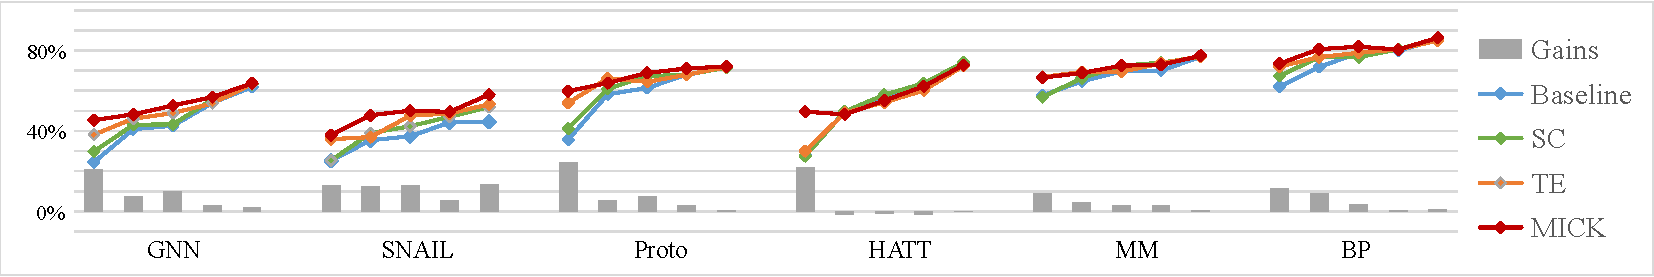
\includegraphics[width=\linewidth]{new51.pdf}
		%\caption{fig1}
	} \\
	\subfigure[5-way 5-shot]{
		\centering
		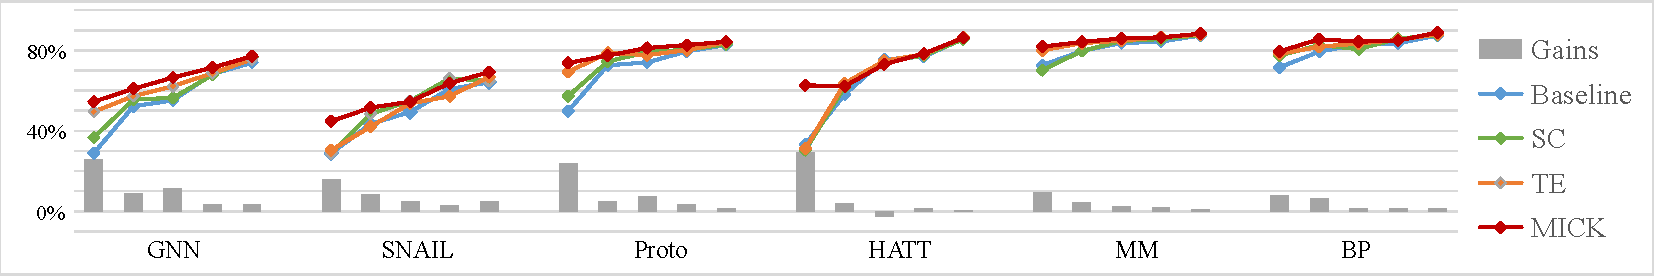
\includegraphics[width=\linewidth]{new55.pdf}
		%\caption{fig2}
	} \\%
	\subfigure[10-way 1-shot]{
		\centering
		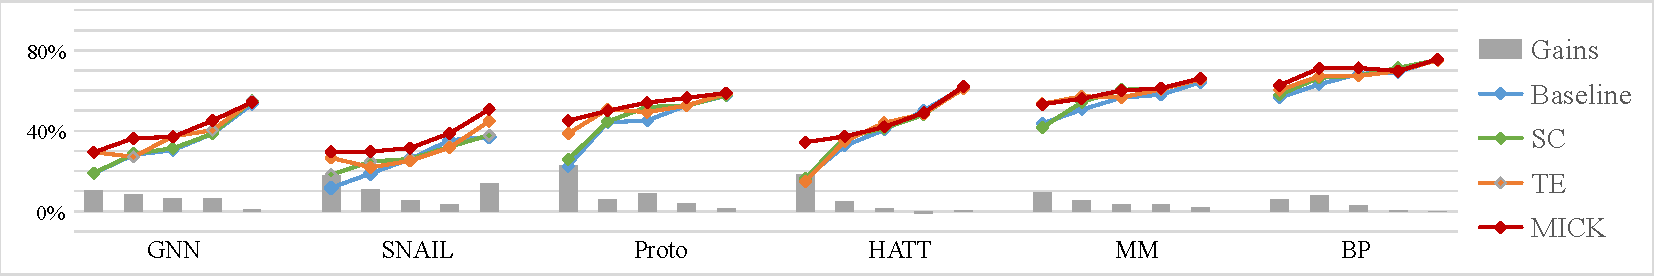
\includegraphics[width=\linewidth]{new101.pdf}
		%\caption{fig2}
	} \\
	\subfigure[10-way 5-shot]{
		\centering
		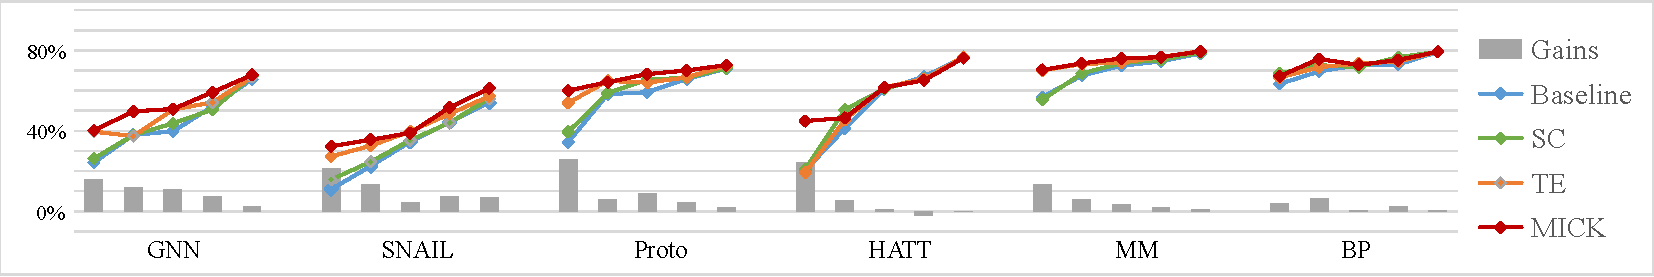
\includegraphics[width=\linewidth]{new105.pdf}
		%\caption{fig2}
	}%
	%\includegraphics[width=0.49\linewidth]{full_results.pdf}
	%%\caption{fig1}
	%}%
	%\subfigure[5-way 5-shot]{
	%\centering
	%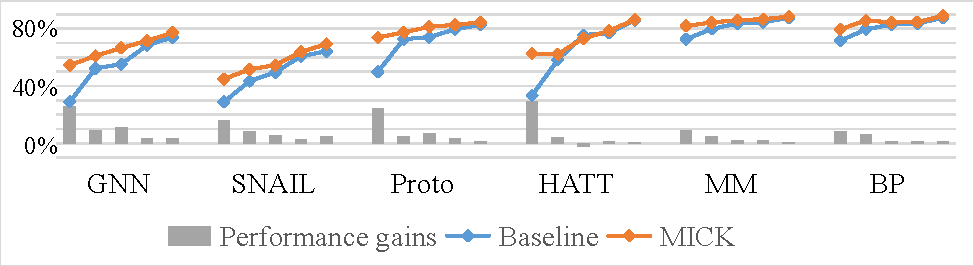
\includegraphics[width=0.49\linewidth]{55.pdf}
	%%\caption{fig2}
	%} \\%
	%\subfigure[10-way 1-shot]{
	%\centering
	%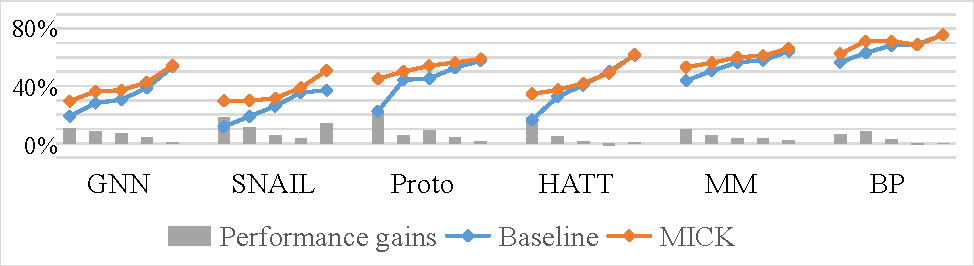
\includegraphics[width=0.49\linewidth]{101.pdf}
	%%\caption{fig2}
	%}%
	%\subfigure[10-way 5-shot]{
	%\centering
	%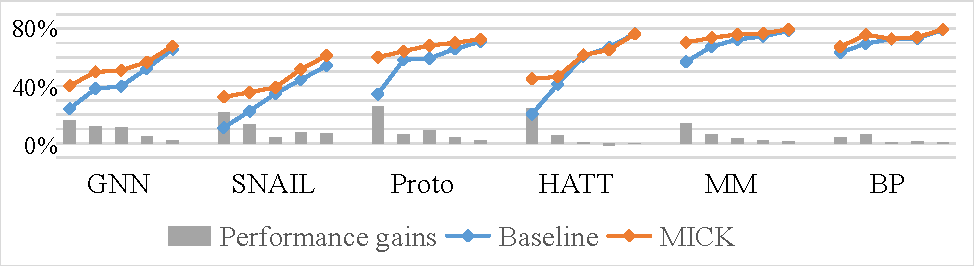
\includegraphics[width=0.49\linewidth]{105.pdf}
	%%\caption{fig2}
	%}%
	
	\centering
	\caption{Classification accuracy on FewRel validation set %with training data shrunken 
		under $N$-way $K$-shot configurations. Gains is the difference between MICK accuracy and baseline accuracy.
		For each group, from the left to the right, training data is shrunken to 0.22\%, 1.00\%, 2.23\%, 7.00\%, and 100.00\% of full training set size, respectively. For each shrunken training set, we apply baseline models and models with SC (Support Classifier individually), TE (Task Enrichment individually) and the whole MICK framework. Proto, HATT, MM, and BP stand for Prototypical Networks, Proto-HATT, MLMAN, and Bert-Pair, respectively.}
	\label{fig:analysis}
\end{figure*}


\subsection{Results and Analysis}
\label{results}
%\KZ{Put more analysis in this section. Make more observation and explain
%things more thoroughly.}
Here, we show the experimental results and analyze them from different aspects.

\subsubsection{With small training data}
To show the effectiveness of our MICK framework under small training data,
we apply it on each baseline model on
(1) FewRel dataset with training set shrunken to different extents, and (2) our proposed TinyRel-CM dataset.

\begin{table*}[th]
\centering
\small
\caption{Classification accuracy (\%) on TinyRel-CM dataset under
	$N$-way $K$-shot configuration.
	% For each cell, $K$=5, 10, and 15 from the top row to the bottom row. 
	D, S, F, and U stand for Disease, Symptom, Food, and nUtrient, respectively.
	Proto, HATT, MM, and BP stand for Prototypical Networks, Proto-HATT, MLMAN, and Bert-Pair, respectively.
	Gray numbers indicate the accuracy is lower than baseline.}
%Meta Networks, SNAIL, GNN, SNAIL and Proto-HATT require the number of classes while training and testing to be equal. So a model is trained with N way tasks to perform N way tests. For SNAIL, the number of instances per relation while training and testing need to be equal. So a model is trained with K shot tasks to perform K shot test tasks.}
\label{FRMresult}
\begin{tabular}{|c|c|cccccc|cccccc|}
\hline
\textbf{Method} & &\multicolumn{6}{c|}{\emph{Baseline}} &\multicolumn{6}{c|}{\emph{+SupportClassifier}} \\ \hline
&\textbf{Group} & D-D & D-S & D-F & D-U & F-U & S-F& D-D & D-S & D-F & D-U & F-U & S-F\\
&\textbf{(N)} & (5) & (2) & (6) & (6)& (2) & (6)& (5) & (2) & (6) & (6)& (2) & (6)\\ \hline
%\multirow{3}{*}{MetaN}      &&&&&& &&&&&& &&&&&& &&&&&&\\
% &&&&&& &&&&&& &&&&&& &&&&&& \\
%&&&&&& &&&&&& &&&&&& &&&&&& \\ \hline
\multirow{3}{*}{GNN}   & (K=~5~)   & 24.04&53.62 &34.15 &38.90 & 54.60& 32.45 &25.71&57.12&33.11&40.23&\textcolor[rgb]{0.45,0.45,0.45}{53.20}&34.51 \\
 & (K=10) & 26.05& 53.73&37.54 &44.02 &\textbf{55.53} &35.45 &\textbf{27.96}&57.35&37.44&43.87&\textcolor[rgb]{0.45,0.45,0.45}{54.85}&\textbf{38.39} \\
 & (K=15) & 26.94& 54.30&38.36 &45.12 &55.45 &37.43 &\textbf{28.36}&61.25&39.18&47.57&\textcolor[rgb]{0.45,0.45,0.45}{55.10}&\textbf{40.37}\\ \hline
\multirow{3}{*}{SNAIL}
 & (K=~5~) &21.74 & 50.00 &17.78 &25.98 & 47.96& 25.38     &23.64&53.90&27.28&27.60&53.15&25.88\\
  & (K=10) & 19.49 & 53.57&27.55 &22.96 &51.63 &22.51      &23.98&56.65&27.76&30.10&54.60&26.10 \\
 & (K=15) & 21.94& 51.62&20.03 &18.21 &50.33 &21.38         &23.12&\textbf{57.40}&27.72&31.43&\textbf{56.35}&25.40\\ \hline
\multirow{3}{*}{Proto}      & (K=~5~)  & 30.03&63.27 &31.35 &33.95 & 54.99& 26.97 &28.99 &\textbf{69.56} &33.57 & 43.78&56.49 &36.81\\
 & (K=10) & 31.68& 67.22&34.09 &36.27 &56.78 &29.18 &32.35 &\textbf{72.54} &36.10 & 47.78& 58.13&39.04\\
 & (K=15) & 33.80& 70.29&34.57 &37.41 &57.03 &29.72 &34.82 &\textbf{72.79} &36.96 &\textbf{50.03} &\textbf{ 60.09} &40.09\\ \hline

% D-D | D-S | D-F | D-U | F-U | S-F %
\multirow{3}{*}{HATT}
 & (K=~5~) &29.67&59.27&40.13&40.19&65.20&41.67  % baseline	5
&36.39&71.45&40.83&\textbf{54.17}&70.09&43.33 \\% cls + data  5
% -------
 & (K=10) &34.50&59.77&39.17&48.33&67.50&43.57  % baseline    10
&40.10&\textbf{71.24}&45.34&50.83&73.33&\textbf{49.17} \\% cls + data  10
% -------
 & (K=15) &39.01&63.75&37.41&\textbf{56.67}&66.25&37.13  % baseline	15
&43.05&77.09&44.17&\textcolor[rgb]{0.45,0.45,0.45}{51.67}&\textcolor[rgb]{0.45,0.45,0.45}{63.75}&45.92  % cls			15
\\% cls + data  15
\hline

\multirow{3}{*}{MM}   & (K=~5~)     &31.22 &60.58 &44.97 &47.11 &61.04 &44.78 &33.48 &62.34 & \textcolor[rgb]{0.45,0.45,0.45}{44.93}&49.49 &62.40 &45.90\\
 & (K=10) & 36.66&64.96 &49.44 &52.49 &66.68 &50.57 &38.89 & 67.30& 50.09& 54.09&68.39 &50.77\\
 & (K=15) & 40.65&68.14 &52.44 &56.00 &70.32 &53.13 &43.05 & 69.41&53.82 &57.23 &72.02 & \textcolor[rgb]{0.45,0.45,0.45}{52.87}\\ \hline
\multirow{3}{*}{BP}  & (K=~5~)    & 23.61&53.48 &46.02 &42.03 & 54.17& 46.18&   24.60 &\textcolor[rgb]{0.45,0.45,0.45}{53.98}&50.49 &\textbf{43.28}&\textbf{63.33}&48.75 \\
 & (K=10) & 24.17& 56.95&49.52 &44.37 &59.72 &48.96 &26.69&\textcolor[rgb]{0.45,0.45,0.45}{55.05} &53.60 &\textbf{46.13}&\textbf{66.70} &51.63  \\
 & (K=15) & 25.80& 54.15&50.38 &45.16 &59.33 &48.78 &27.29 &56.65 &54.22&\textbf{47.81} &67.55 &52.48 \\ \hline
%\multirow{3}{*}{BP2}      & \emph{K=~~5} & 21.83&52.52 &28.73 &30.68 & 54.69& 27.79 &&&&&& &&&&&& &&&&&&\\
%& \emph{K=10} & 22.15& 53.34&32.15 &34.52 &55.20 &30.95 &&&&&& &&&&&& &&&&&&\\
%& \emph{K=15} & 21.56& 54.83&33.74 &36.95 &55.99 &33.00 &&&&&& &&&&&& &&&&&&\\ \hline
%\hline

\textbf{Method} & & \multicolumn{6}{c|}{\emph{+TaskEnrich}} &\multicolumn{6}{c|}{\emph{+SupportClassifier\&TaskEnrich}} \\ \hline
& \textbf{Group} & D-D & D-S & D-F & D-U & F-U & S-F& D-D & D-S & D-F & D-U & F-U & S-F\\
& \textbf{(N)} & (5) & (2) & (6) & (6)& (2) & (6)& (5) & (2) & (6) & (6)& (2) & (6)\\ \hline
\multirow{3}{*}{GNN}
 & (K=~5~) & 24.59&\textcolor[rgb]{0.45,0.45,0.45}{51.20}&\textcolor[rgb]{0.45,0.45,0.45}{33.28}&40.76&54.62&35.36 &\textbf{26.02}&\textbf{66.22}&\textbf{37.48}&\textbf{44.47}&\textbf{55.02}&\textbf{37.13} \\
 & (K=10) &26.85&56.05&37.56&44.90&\textcolor[rgb]{0.45,0.45,0.45}{54.12}&37.69 &27.66&\textbf{58.75}&\textbf{37.88}&\textbf{45.15}&\textcolor[rgb]{0.45,0.45,0.45}{53.42}&37.85 \\
 & (K=15) &27.71&58.55&40.42&49.43&56.35&40.13 &27.40&\textbf{70.10}&\textbf{43.25}&\textbf{51.40}&\textbf{56.45}&40.03 \\ \hline
\multirow{3}{*}{SNAIL}
 & (K=~5~) &22.43&53.95&25.17&\textbf{29.05}&51.30&27.27&\textbf{24.64}&\textbf{58.55}&\textbf{28.57}&27.08&\textbf{53.30}&\textbf{27.88} \\
 & (K=10) &22.79&\textcolor[rgb]{0.45,0.45,0.45}{51.98}&\textbf{30.67}&\textcolor[rgb]{0.45,0.45,0.45}{22.13}&53.15&23.03         &\textbf{27.38}&\textbf{57.12}&\textbf{27.85}&\textbf{33.50}&\textbf{55.60}&\textbf{30.52} \\
 & (K=15) &\textcolor[rgb]{0.45,0.45,0.45}{21.54}&53.10&20.77&\textbf{20.35}&52.00&23.30     &\textbf{23.84}& 56.70&\textbf{30.63}&\textbf{35.75}&54.30&\textbf{30.43} \\ \hline

\multirow{3}{*}{Proto}
 & (K=~5~) &31.40 &69.22 &32.13& 34.22&55.34&30.34&\textbf{31.50} &68.79 &\textbf{34.36} & \textbf{44.76} &\textbf{57.43}&\textbf{40.36} \\ 
 & (K=10) &34.80 &72.34 &34.51&36.58&57.29&33.81&\textbf{35.45} &71.37 &\textbf{37.11} & \textbf{48.28}&\textbf{58.71}&\textbf{43.55} \\
 & (K=15) &36.97 &71.62 &35.76 &37.79 &57.74&34.49&\textbf{38.28} &72.62 &\textbf{37.90} &49.58 &60.00&\textbf{44.97} \\ \hline

\multirow{3}{*}{HATT}
 & (K=~5~) &33.70&67.50&41.67&43.33&65.62&\textcolor[rgb]{0.45,0.45,0.45}{38.33} &\textbf{38.21}&\textbf{75.00}&\textbf{46.67}&49.17&\textbf{73.75}&\textbf{44.17} \\
 & (K=10) &38.98&68.75&40.13&48.75&\textcolor[rgb]{0.45,0.45,0.45}{60.92}&46.67  % data        10
&\textbf{44.45}&70.23&\textbf{49.37}&\textbf{51.67}&\textbf{75.00}&44.47 \\
 & (K=15) &40.39&72.31&43.84&\textcolor[rgb]{0.45,0.45,0.45}{55.83}&70.51&43.33  % data		15
&\textbf{49.61}&\textbf{80.41}&\textbf{44.33}&\textcolor[rgb]{0.45,0.45,0.45}{55.81}&\textbf{72.58}&\textbf{49.17} \\ \hline

\multirow{3}{*}{MM}
 & (K=~5~) &36.05 & \textbf{64.98}& 45.24&50.03 &61.34 & 46.82&\textbf{38.17} &64.68 & \textbf{45.32}& \textbf{51.30}& \textbf{64.24}& \textbf{48.34} \\
 & (K=10) &42.04 & \textbf{70.02}& \textbf{50.83} &54.85 &67.57 &52.47&\textbf{44.89} &69.93 & 50.75& \textbf{56.60}& \textbf{70.79} &\textbf{53.69} \\ 
 & (K=15) &46.55& 71.95&54.18 &58.19 &72.01 &55.28&\textbf{49.23} & \textbf{72.41}& \textbf{54.25}& \textbf{59.67}& \textbf{74.58}& \textbf{56.67} \\ \hline

\multirow{3}{*}{BP}
 & (K=~5~) &25.25&\textbf{59.52}&48.49&\textcolor[rgb]{0.45,0.45,0.45}{40.32}&55.73&48.68 &\textbf{26.87}&58.35&\textbf{52.54}&\textcolor[rgb]{0.45,0.45,0.45}{39.48}&62.52&\textbf{49.95} \\
 & (K=10) &27.54&61.48&51.11&\textcolor[rgb]{0.45,0.45,0.45}{44.33}&60.15&51.56 &\textbf{28.19}&\textbf{62.32}&\textbf{55.86}&\textcolor[rgb]{0.45,0.45,0.45}{43.25}&66.38&\textbf{52.92} \\
 & (K=15) &28.29&\textbf{63.98}&52.18&47.32&61.02&53.36 &\textbf{29.25}&63.15&\textbf{57.60}&\textcolor[rgb]{0.45,0.45,0.45}{43.26}&\textbf{68.83}&\textbf{54.16} \\ \hline
\end{tabular}
\end{table*}


Figure \ref{fig:analysis} shows the performance comparison between baseline models and our framework given different amount of training data on FewRel dataset. 
Each subgraph contains 6 groups, one group for each baseline model. For each group, the training data size increases from the left to right. 
Here, we focus on the blue curves which present baseline accuracies, the red curves which present the MICK enhanced model accuracies, and the gray bars which present the performance gains that MICK brings.
As is illustrated, performance of models deteriorates with the decrease of training data size. For example, the prototypical networks achieves 57.53\% accuracy with full training data under 10-way 1-shot test tasks, but performs poorly with 22.30\% accuracy given only 0.22\% of full training data.
Our framework fits in situations where only small training data is available. As is shown in Figure \ref{fig:analysis}, with our methods, the less the training data, the more improvement the model tends to gain. This indicates the effectiveness of our framework under extremely small training data. While our methods only improve prototypical networks by 1.27\% accuracy with full training data under 10-way 1-shot test tasks, it leads to 22.74\% improvement given 0.22\% of full training data.
%When the input sentence contains multiple relation classes, model performance drops (by 14.14\% under 2.23\% full FewRel training data under 5-way 5-shot tasks using MLMAN). 

Table \ref{FRMresult} shows the experimental results on the TinyRel-CM dataset.
Our framework considerably improves model performance in most cases.
Strong baselines on FewRel dataset such as Bert-Pair do not perform well, partially because the TinyRel-CM dataset is more verbal and informal, thus quite distinct from BERT-Chinese's pretraining data (Chinese Wikipedia).

On both datasets, when the input sentence contains multiple relation classes, model performance drops. E.g., under 2.23\% full FewRel training data under 5-way 5-shot tasks using MLMAN, classification accuracy on relation class \emph{mother} decreases by 14.14\% when \emph{spouse} or \emph{child} appears as interference.

\subsubsection{With sufficient training data}

We use full training data from FewRel dataset and apply MICK framework on each baseline model.

Here, we focus on the rightmost blue points, red points and gray bars of each group in \figref{fig:analysis}, which present the baseline performance, MICK performance and performance gains brought by MICK under full FewRel training data. As is shown in \figref{fig:analysis}, on full FewRel dataset, in most cases, our framework achieves better performance than baseline models.
The framework brings more improvement for relatively poor baselines such as GNN and SNAIL (about 5\% accuracy) than strong baselines such as MLMAN and Bert-Pair (about 1\% accuracy). This is because our framework aims to help models learn better and doesn't change the core part of the models. Full training data is sufficient for strong baselines to train a good model, leaving limited room for improvement. 
%However, we show in \figref{fig:analysis} that by cutting down the training data size, the advantage of our framework is apparent.



% \subsubsection{FewRel dataset with reduced training data}
%Table \ref{FewRelval} shows the experimental results on the FewRel dataset. We either keep the original training set or shrink the training set to different extents and test on the validation set. Table \ref{FewRelval} illustrates the strength of our framework and data augmentation method since performance gains are attained in most cases. While the MSI framework keeps helping models to leaner better, data augmentation tends to be more effective when training data is quite limited.
%Figure \ref{fig:analysis} shows the performance gains on MLMAN using MSI framework and data augmentation. The less the training data, the more improvement the model gains, indicating that the MSI framework and data augmentation method's effectiveness under extremely limited training data.




\subsubsection{Ablation tests}

Here, we focus on the individual effects of support classifier and task enrichment on baseline models. %We facilitate baseline models with either MSI framework or data augmentation and compare the performance with both baseline models and models with

As is shown in Figure \ref{fig:analysis} and Table \ref{FRMresult}, in most cases, either adding support classifier or task enrichment improves performance for baseline models.
%and either removing support classifier or data augmentation leads to performance decrease from the models trained with both methods.
This illustrates that both support classifier and task enrichment contribute to better performance.

On FewRel dataset, we focus on the green and orange curves in \figref{fig:analysis}, which present the accuracies of applying support classifier or task enrichment individually.
% Support classifier
Support classifier generally brings more performance gains when less training data is given. This is because with small training data, baseline models fail to extract adequate knowledge while the support classifier helps with the knowledge learning process.
In some rare cases such as SNAIL under 5-way 1-shot and 5-way 5-shot scenarios with 0.22\% training data, adding support classifier leads to not much improvement. 
This is because support classifier guides models to extract more knowledge from very limited resources, while the extractable knowledge is restricted by the training set size and some of the knowledge is even useless.
Support classifier improves poor baselines such as GNN and SNAIL to a larger extent than strong ones such as MLMAN and Bert-Pair because the support classifier makes up for the insufficient learning ability for poor models while is icing on the cake for strong models. %with sufficient training data.

%TE
Task enrichment is much more helpful than support classifier under small training data (when training data is shrunken to less than 1.00\%). This is because task enrichment compensates for the lack of learning sources of basic knowledge such as basic rules and grammar when training data is quite limited.
Improvement of task enrichment is also more obvious on poor baselines than strong ones. Since poor models fail to master some of the basic knowledge brought in original training data, the introduction of cross-domain data not only brings extra basic knowledge but also helps models to master knowledge in original training data by providing more related data.
%provides more learning resources and help the models learn better about basic knowledge. 

Applying both support classifier and task enrichment achieves best performance in most cases, because the two methods complement each other. Support classifier extract useful information from original training data and cross-domain data, and task enrichment provide extra sources for the support classifier. %knowledge from both original training set and cross-domain data are fully extracted. 
In some cases, although adding either support classifier or task enrichment does not affect much, applying them together leads to a great improvement (e.g., HATT under 0.22\% training data).
%When applied together, support classifier leads to more gains when applied on task enriched models. Because cross-domain data may lead to noise while support classifier helps to choose what to learn.

%Both support classifier and task enrichment bring more performance gains for poor baselines such as GNN and SNAIL than strong ones such as MLMAN and Bert-Pair. 
%Support classifier is more powerful on poor models because the support classifier makes up for the insufficient learning ability for poor models while is icing on the cake for strong models with sufficient training data.
%Improvement of task enrichment is also more obvious on poor baselines than strong ones. Since poor models fail to master basic knowledge such as basic rules and grammar, the introduction of cross-domain knowledge provides more learning resources and help the models learn better about basic knowledge. While for strong models that already learn basic knowledge well, cross-domain task enrichment may bring in noise because of distinct data distributions. This is why sometimes task enrichment brings negative gains.
%stable on strong baselines while fluctuates on poor ones. This reflects the unstableness of poor baselines. With defects in learning ability, supplementary data brings harder tasks and may confuse poor models, and this is why sometimes data augmentation brings negative gains.

On TinyRel-CM dataset (\tabref{FRMresult}), %the improvement is more obvious with either support classifier or task enrichment than on FewRel dataset because of more room for progress.
task enrichment brings about similar improvements for all baselines due to small training data. Support classifier leads to more performance gains than task enrichment individually,
indicating TinyRel-CM dataset is more challenging (the relation classes are much more similar than FewRel dataset) and baseline models fail to extract sufficient useful knowledge.
%indicating model's learning ability is more essential than extra knowledge. 
Although task enrichment brings not much improvement or even negative effects in some cases, adding support classifier simultaneously tend to raise the accuracy to a large extent (up to 10\%). 
The reason is that with insufficient learning ability %(including strong baselines such as MLMAN and Bert-Pair under small data size \KZ{On the one hand you said insufficient learning ability, on the other
%hand you said strong baseline, contradiction?}),
(although baselines such as MLMAN and Bert-Pair are relatively strong, their learning ability is still insufficient with small training data),
cross-domain data alone sometimes introduces
noise and thus confuses the model. But with the additional support classifier
that improves learning ability, models are able to learn more useful
knowledge from cross-domain data.
%This is because with poor learning ability (although baselines such as MLMAN and Bert-Pair are strong on FewRel dataset, their learning ability is still unsatisfying under such small data size), cross-domain data sometimes make things tougher and may confuse the model, while with support classifier which improves learning ability, models are able to learn useful knowledge from cross-domain data.

On %both FewRel dataset (\tabref{FewRelvalAll}) and
TinyRel-CM dataset (\tabref{FRMresult}), few cases occur where adding both support classifier and task enrichment performs worse than adding only one of them
(e.g., Bert-Pair under group D-U, and prototypical networks under group D-S in TinyRel-CM dataset).
The main reason is that while adding the support classifier helps models learn more and better, the model occasionally tend to pay excessive attention to the distinctive distribution of the cross-domain data.
As is shown in the corresponding results, in the vast majority of cases, while adding support classifier on baseline models raises accuracy, adding support classifier on task enriched models brings less improvement or even bad effect. This indicates stronger learning ability owing to the support classifier, and the distraction caused by cross-domain data.

\begin{table}[ht]
	\centering
	\small
	\caption{Human evaluation result on TinyRel-CM dataset under 5-shot scenario.}
	\label{human}
	\begin{tabular}{|c|cccccc|}
		\hline
		\textbf{Group} & D-D & D-S & D-F & D-U & F-U & S-F \\
		\textbf{(N)} & (5) & (2) & (6) & (6) & (2) & (6) \\ \hline
		\textbf{Acc(\%)} & 92.65 &96.53 & 86.93 & 91.77 & 96.71& 84.97\\ \hline
	\end{tabular}
\end{table}

\subsubsection{Dataset analysis}
Our TinyRel-CM dataset is a challenging task.
We human evaluate the dataset and results are illustrated in Table \ref{human}.
During the human-evaluation process, under $N$-way $K$-shot scenario, we provide instances of $N$ relation classes with $K$ instances per relation class. We use labels $1$ to $N$ to name the relation classes instead of their real names. A person is required to classify a new coming instance into one of the $N$ classes. 
We only evaluate the TinyRel-CM dataset under 5-shot scenarios because 10-shot and 15-shot tasks are too easy for human.
Three volunteers participated in the human evaluation process and we take the average accuracy as the final result.

Comparing Table \ref{FRMresult} and Table \ref{human}, the performance of state-of-the-art models is still far worse than human performance, indicating the TinyRel-CM dataset is a challenging task.


%Our TinyRel-CM dataset is more challenging than FewRel dataset.
%The TinyRel-CM dataset has two major difficulties.
%One is the tiny training data size. As is shown in \figref{fig:analysis}, as the training data shrinks, the performance of each model drops evidently. This indicates the less the training data, the more challenging the task becomes.
%
%The other difficulty is that, in TinyRel-CM dataset, given any test task, head and tail entity types of each relation class are the same. This makes the TinyRel-CM dataset more challenging than FewRel dataset even with similar amount of training data.
%Comparing \tabref{FRMresult} and \figref{fig:analysis}, taking baseline MLMAN as an example, MLMAN achieves over $80\%$ accuracy under 5-way 5-shot configuration with $2.23\%$ of full FewRel training data (20 classes with 50 instances per class), while only $31.22\%$ accuracy under 5-way 5-shot configuration (D-D group) with TinyRel-CM dataset (22 classes with 50 instances per class as training set).
%
%To confirm this issue, we choose relation class \emph{mother}, the head and tail entity types of which are \emph{PERSON1} and \emph{PERSON2}, in FewRel dataset as a sample for further analysis. We compute two accuracies: (1) Distinct entity type accuracy: classification accuracy of relation class \emph{mother} without any other candidate relation classes whose target entity types are \emph{PERSON1} and \emph{PERSON2}, and (2) Same entity type accuracy: classification accuracy of \emph{mother} where \emph{spouse} or \emph{child} is among the candidate classes in the same task. We do this analysis under three typical baseline models: prototypical networks, MLMAN and Bert-Pair. We conduct 5-way 5-shot test configuration under $2.23\%$ full training data (20 classes with 10 instances per class). Results are shown in \tabref{etypeanalysis}.  As is illustrated, the accuracy of \emph{mother} accompanied by \emph{spouse} or \emph{child} is much lower than the accuracy of \emph{mother} without same-entity-type classes, indicating shared target entity types among candidate classes brings challenge to models.
%Only two relation classes with the same target entity types raise such difficulty, not to mention the TinyRel-CM dataset where all candidate classes have common target entity types.
%
%\begin{table}[ht]
%\centering
%\small
%\caption{5-way 5-shot classification accuracy (\%) on relation class \emph{mother} in FewRel dataset.
%	Etype stands for Entity type.
%	%Distinct etype represents classification accuracy with other candidate classes that have distinct target entity types with \emph{mother}.
%	%Same etype represents classification accuracy where some candidate classes share same target entity types with \emph{mother}.
%	Proto, MM, and BP stand for Prototypical Networks, MLMAN, and Bert-Pair, respectively.}
%\label{etypeanalysis}
%\begin{tabular}{|c|p{56pt}<{\centering}|p{56pt}<{\centering}|}
%\hline
%\textbf{Method} &\textbf{Distinct Etype} & \textbf{Same Etype} \\ \hline
%Proto & 77.91 & 63.39 \\
%MM & 86.84 & 72.70 \\
%BP & 96.89& 54.67 \\ \hline
%\end{tabular}
%\end{table}



\section{Related Work}
%\subsection{Relation Classification}
%\KZ{Reduce this section}
%Relation classification task aims to categorize the semantic relation between two entities conveyed by a given sentence into a relation class.
%In recent years, deep learning has become a major method for relation classification.
%\cite{RecursiveNNRC} fed the recurrent neural network (RNN) with a syntactic tree to introduce attention mechanism in relation classification tasks. \cite{zeng-etal-2014-relation} utilized a convolutional deep neural network (DNN) during relation classification to extract lexical and sentence-level features. \cite{vu-etal-2016-combining} employed a voting scheme by aggregating a convolutional neural network with a recurrent neural network.
%
%Traditional relation classification models suffer from lack of data. To eliminate this deficiency, distant-supervised approaches are proposed, which take advantage of knowledge bases to supervise the auto-annotation on massive raw data to form large datasets. \cite{NYTdataset} constructed the NYT-10 dataset with Freebase \cite{Freebase} as the distant supervision knowledge base and sentences in the New York Times (2005-2007) as raw text. Distant-supervised methods suffer from long tail problems and excessive noise. \cite{zeng-etal-2015-distant} proposed piecewise convolutional neural networks (PCNNs) with instance-level attention to eliminate the negative effect caused by the wrongly labeled instances on NYT-10 dataset. \cite{liu-etal-2017-soft} further introduced soft label mechanism to automatically correct not only the wrongly labeled instances but also the original noise from the distant supervision knowledge base.

%Relation classification task aims to categorize the semantic relation between two entities conveyed by a given sentence into a relation class.
Few-shot relation classification is a newly-born task that requires models to do relation classification under merely a few support instances. Han et al. \shortcite{han-etal-2018-fewrel} proposed the FewRel dataset for few-shot relation classification and applied meta-learning methods intended for CV \cite{metanet,gnn,snail,proto} %with CNN and PCNN core
on the FewRel dataset.
Meta Networks \cite{metanet} implemented a high level meta learner based on the
conventional learner.
GNN \cite{gnn} regarded support and query instances as nodes in a graph.
SNAIL \cite{snail} aggregated attention into the meta learner.
Prototypical networks \cite{proto} assumed that each relation has a prototype and classifies a query instance into the relation of the closest prototype.
Prototypical networks \cite{proto} with CNN core turned out to have the best test accuracy among the reported results. ProtoHATT \cite{hatt} reinforced the prototypical networks with hybrid attention mechanism. MLMAN \cite{ye-ling-2019-multi} improved the prototypical networks by adding mutual information between support instances and query instances. Bert-Pair \cite{gao-etal-2019-fewrel} adopted BERT \cite{devlin2018bert} to conduct binary relation classifications between a query instance and each support instance and fine-tune on FewRel dataset. Baldini Soares et al. \shortcite{baldini-soares-etal-2019-matching} trained a BERT-like language model on huge open-source data with a Matching the Blanks task and applied the trained model on few-shot relation classification tasks.

Meta networks performs worst among all the methods \cite{han-etal-2018-fewrel} and
is time consuming (about 10 times slower than other methods with even better results).
%\KZ{How time-consuming? Better give some numbers. And then say that's why
%we didn't include it in our experiments.} % due to the complex training strategy.
Matching the Blanks is high-resource and not comparable to other methods. So we do not adopt these two methods as baselines.
%\subsection{Meta-learning}
% in CV... 组会的papers!
%Meta-learning aims to .... It is first proposed by [??] where the authors ...image classification... and is widely researched in computer vision. One category of meta-learning methods trains a meta-learner above the traditional learner. The meta-learner guides the learning steps of the traditional learner[?? ??]. Another category bases on metric learning, which aims to find the underlying distribution among all the classes[?? ??]. Prototypical networks[??] is a typical framework of metric-learning based meta-learning. It proposes the concept of prototype, which is a centroid among all the support vectors within the same class, and uses the prototypes to represent the vectors of each relation. In [??], prototypical network is adopted to handle NLP tasks such as few-shot relation classification.

%The methods of updating models in previous works rely on the output of the query instances to a great extent, which lose sight of the significant and precious information within the support instances.
Previous methods lose sight of the significant information within the support instances.
Chen et al. \shortcite{chen-2019-image} conducted image one-shot learning tasks with a image deformation sub net and trained a prototype classifier to classify the prototypes of the support instances to update the parameters within the image deformation sub net. Inspired by this work, we add a support classifier over each support instance during the training process. The support classifier helps with the update process of the parameters in both the support classifier and the encoder, and is scheduled with a fast-slow learner schema.


%\subsection{Datasets}
%Relation classification datasets have been released in past decades. Conventional ones include SemEval-2010 Task 8 dataset \cite{semeval8}, ACE 2003-2004 dataset \cite{ace}, TACRED dataset \cite{zhang-etal-2017-position} and NYT-10 dataset \cite{NYTdataset}. All these datasets encompass sufficient data to train a strong model.
Han et al. \shortcite{han-etal-2018-fewrel} released the first few-shot relation classification dataset, the FewRel dataset, which contains 100 relation classes with 700 instances per class. Although the dataset is intended for few-shot relation classification, the training data is still adequate.
% (the model meets 700 instances times 100 classes during training). % And the performance of models decrease if the training data decreases.
We propose TinyRel-CM dataset, which is a \emph{real} few-shot relation classification dataset with 27 classes and only 50 instances per class. The TinyRel-CM dataset is a much harder task than the previous dataset.
%few-shot relation classification tasks. %In our paper, we also propose a method that is capable of handling few training data.


\section{Conclusion}
In this paper, we propose a few-shot learning framework for relation classification that aims to extract information within support instances and using data augmentation. Our methods are extremely powerful under circumstances where limited training data is available.
%MME aims to extract underlying information brought within support sentences. In MME, a supplementary classifier is adopted to classify the relation of each support sentence, and participates in the back propagation progress by a fast-slow learner strategy. We also propose a way of aggregating cross-domain data into the training process. This helps the model to learn underlying cross-domain knowledge. These two innovations are especially useful under circumstances where extremely few data is available.
Additionally, we construct our own dataset, the TinyRel-CM dataset, a Chinese few-shot relation classification dataset in medical domain. The small training data size makes the TinyRel-CM dataset a challenging task.
%Different from previous released few-shot relation classification datasets, the TinyRel-CM dataset contains extremely limited labeled data and provides a much harder few-shot learning task. Our proposed MME framework and data augmentation method achieves state-of-the-art accuracy on the TinyRel-CM dataset and competitive results on the FewRel dataset.
%As for future work, we aim to extract abundant relation classes and instances from massive open-source data with our proposed MME framework to construct a knowledge base in medical domain .


%\section{Problems}
Our model is the best among light models.. Matching the blanks.

**Normal method 50 or 15?

CNN+proto vs CNN-ATT /PCNN-ATT ok?

Seems nowhere to mention supplementary data in related works...

Where to say our relations in dataset can be split into groups...

Task formulation: few-shot learning? meta-learning?

Eval on our dataset?

**Only adding classifier seems ...

The standard results are like x+-0.0x Ours:x

How to determine N...?

!!!!!!!renjia pao de training 20*10 wo men dagai pao bu qi lai

**When giving examples, use English or our Chinese dataset? If use others' dataset, add reference or not?

https://thunlp.github.io/fewrel.html .. Test on this dataset!

\end{CJK}

\bibliographystyle{ACM-Reference-Format}
\bibliography{ref}

\end{document}

